
\documentclass[11pt]{article}
\usepackage[margin=1in]{geometry}

% Core packages
\usepackage{amsmath,amssymb}
\usepackage{tikz-cd}
\usepackage{graphicx}
\usepackage{subcaption}
\usepackage{multicol}
\usepackage{csquotes}
\usepackage{booktabs}
\usepackage{pgfplots}
\pgfplotsset{compat=1.18}
\usepackage{xurl}
\usepackage[authoryear,round]{natbib}
\usepackage{hyperref}
\usepackage{array}
\usepackage{longtable}
\usepackage{placeins}

\newcommand{\eqnote}[1]{{\small\itshape #1}\par\addvspace{4pt}}
\newcommand{\dither}{\textnormal{---}}
\newcommand{\eqn}[1]{\eqref{eq:#1}}
\newcommand{\dg}{\textsuperscript{\dag}}
\newcolumntype{L}[1]{>{\raggedright\arraybackslash}p{#1}}
\newcolumntype{K}[1]{>{\raggedright\arraybackslash\ttfamily\footnotesize}p{#1}}
\newcolumntype{S}[1]{>{\raggedright\arraybackslash\footnotesize}p{#1}}

% Allow long URLs and citation strings to wrap within the text block.
\setlength{\emergencystretch}{3em}

% Paragraphs
\setlength{\parindent}{0pt}
\setlength{\parskip}{1\baselineskip}

\title{Draft: Modelling Psychological and Cultural AI Risk Propagation in the Financial System}
\author{Simon G. Thompson}
\date{\today}

\begin{document}
\maketitle


\begin{abstract}
The financial system is a critical component of our society; its functioning determines the well-being of humans everywhere. The financial system is exposed to damage created by disruptive change which impacts its human components. One such change is the development of modern AI and modern AI's impact on human psychology and behaviours, and the knock on impacts on human institutions. The changes to human behaviour and institutions could potentially propagate into the functions of the financial system, changing and impairing them and creating significant harms.

 A specific example of this interaction (the suppression of human learning) is modelled as a computational simulation and a series of experiments using empirical data from recent real world measurements of AI impact on humans are reported. These indicate that the effects currently being measured and described in empirical studies of AI use and AI in education could create long term impairment of global system functions. 

Contribution: a description of how AI could impact the functioning of the financial system via psychological, cultural and institutional mechanisms; a description of an agent based simulation modelling institutional and global learning in the system based on data about the system in 2026 \footnote{the contribution of my research assistant Arwen Thompson is acknowledged for her work gathering information on the component institutions in the graph of the financial system used in the world model tested in this paper}; a demonstration of the impact of the empirical findings by \cite{david_stromberg_generative_2026} and \cite{fabrizio_dellacqua_navigating_nodate} in the simulated system showing how significant long term harm to human knowledge systems emerges if the empirical information we have and the dynamics of our simulation are useful. 
\end{abstract}

\begingroup
\setlength{\parskip}{0pt}
\tableofcontents
\endgroup
\clearpage

\begin{figure}[htbp]
\vspace{-0.75\baselineskip}
\centering
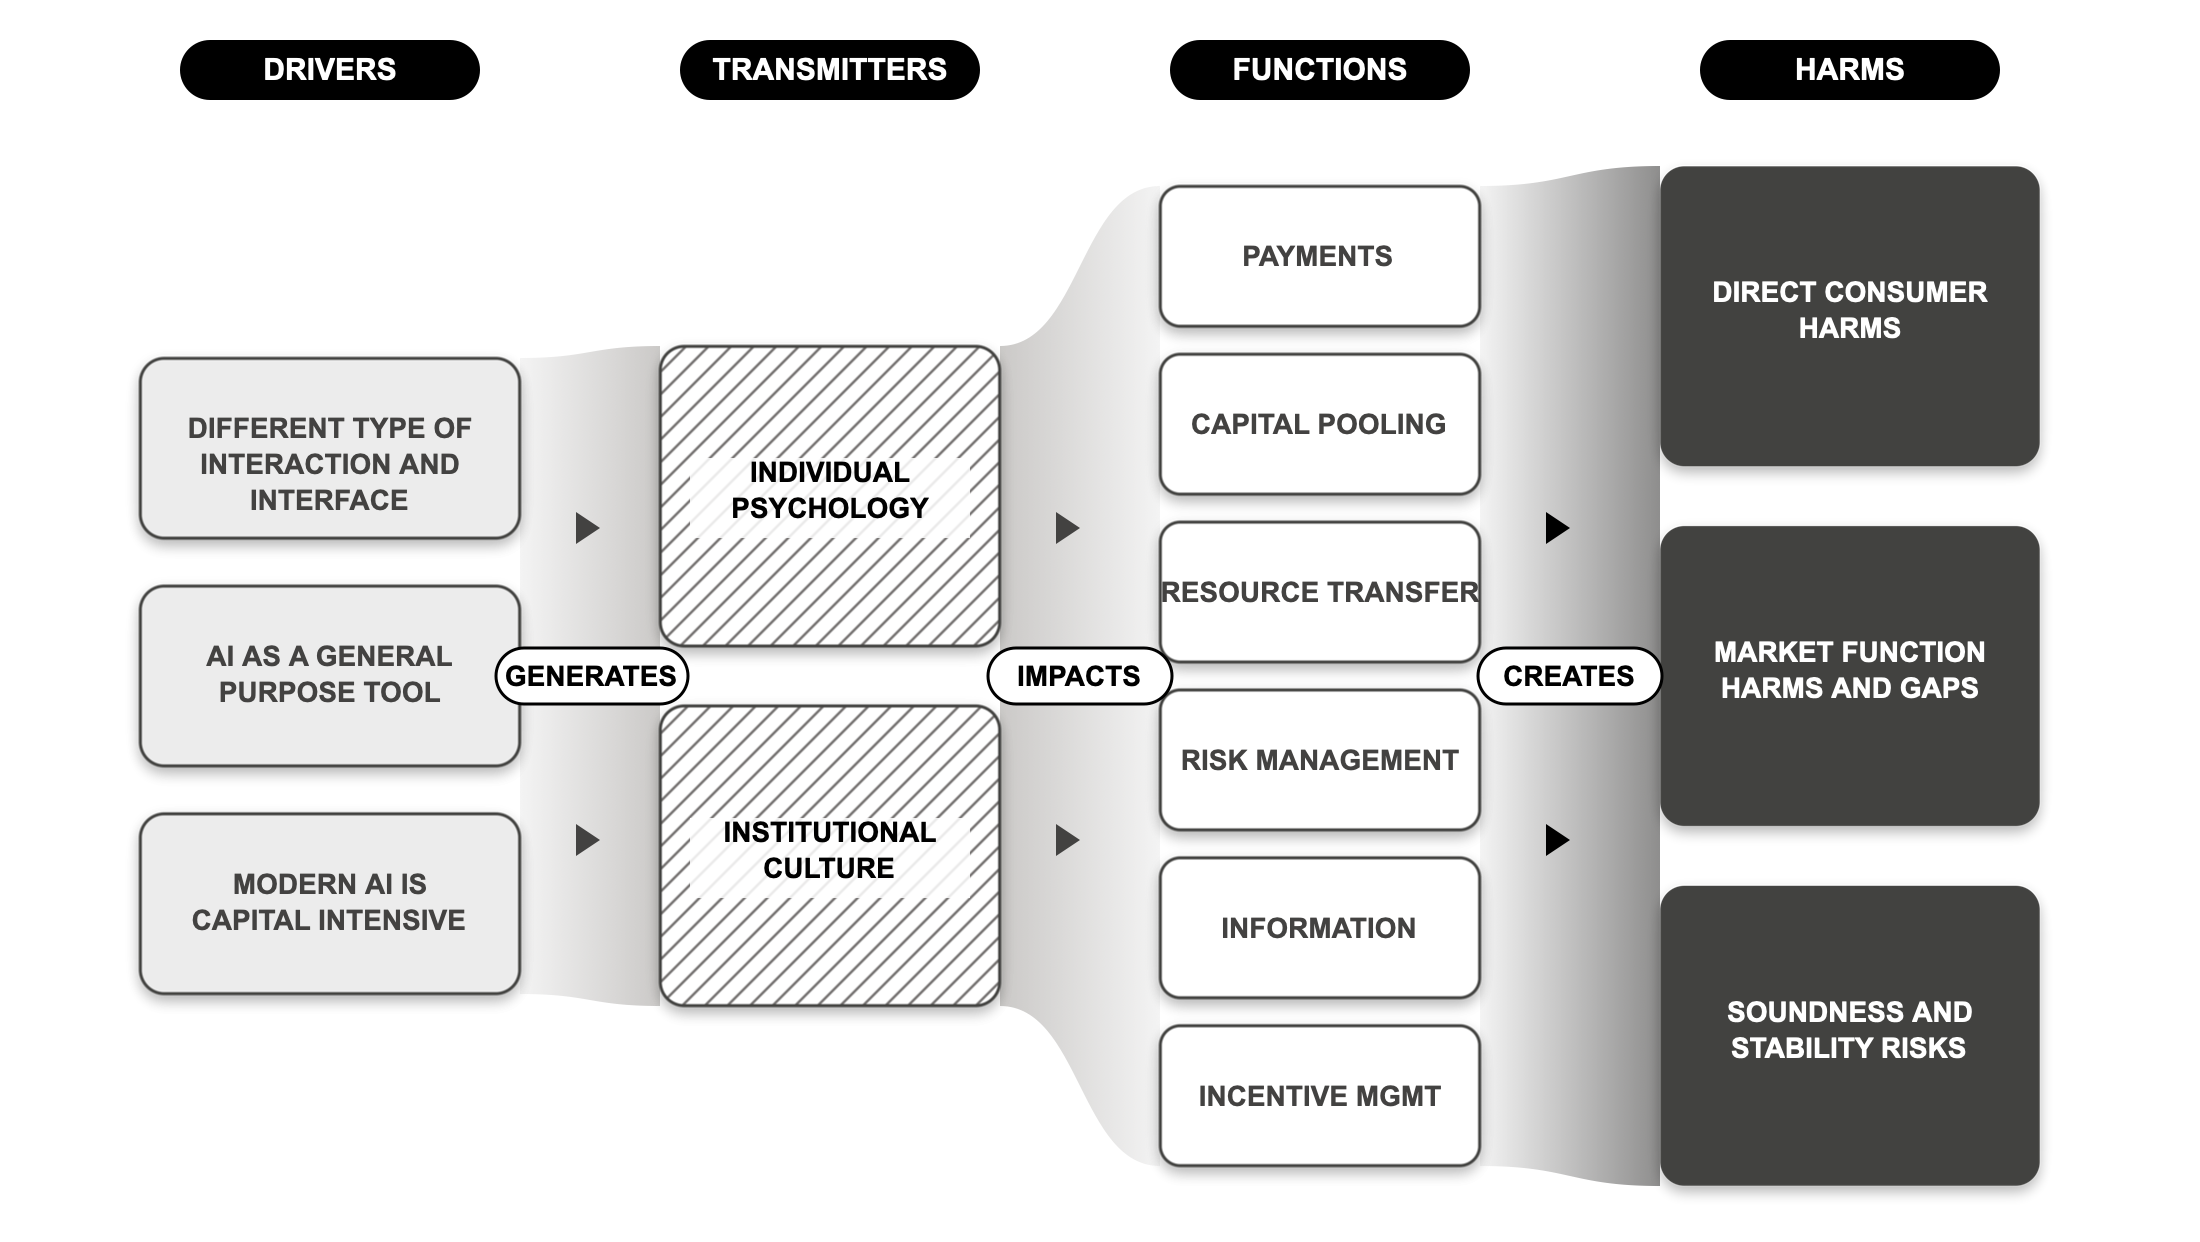
\includegraphics[width=0.85\linewidth]{dynamic-matrix-bw.png}
\caption{How the features of modern AI can change our institutions, creating impacts and propagating as risk to the working of the system. I would like to thank and acknowledge Andrew Sutton, Martin Rusch, and other colleagues and collaborators in the ``Chapter 2 working group'' for their collaboration on the development of the risk propagation idea.}
\label{fig:risk-propagation-model}
\vspace{-0.75\baselineskip}
\end{figure}

\section{Introduction} \label{sec:introduction}

There are many ways that AI\footnote{In this paper AI is broadly defined as modern AI, generative AI, and agentic AI, in contrast to the smaller and more specialised statistical AI models that are developed to solve domain-specific tasks.} could bring down the financial system. For example the FT reports concerns that Claude Mythos will allow hackers to wreck everything. More recently investors in large American AI companies have raised the possibility that open source AI might create significant harms e.g.\footnote{See \url{https://x.com/shaunralston/status/2070947238365499902} where the founder of Anthropic is shown on video talking about how open source models will allow the production of biological weapons.} 

Other, more systemic, mechanisms involve the collapse of private credit due to data centre build outs, and the impact of changing dynamics in pricing, liquidity and trust as AI technology is used to automate and implement components in the system. 

So, there are many possible ways that AI could trouble the financial system but while many commentators lay out possible issues and sometimes are able to identify particular pain points that AI might create in the financial system the mechanisms are often either immediate and catastrophic (and therefore obvious and often resolvable) or vague and redolent of fear, uncertainty and doubt (FUD). Mechanisms that are subtle, long term and potentially irreversible have different characteristics. They are both material and hard to remedy post-facto. AI risks could arise through the mechanics of its impact on human psychology and cognition, and subsequently on the cultures of the institutions that comprise the financial system as we know and recognise it today. The work here describes conceptual and formal models of how these risks might propagate and impact the functioning of the system. The intent of developing these models is to quantify and qualify the mechanisms that might create risk and to identify how these  might be interrupted to create mitigations. 

\section{Approach}\label{sec:approach}

At a high level the flow of impact and risk illustrated in figure \ref{fig:risk-propagation-model} provides a description of why AI could be seen as a dangerous technology that requires some management. This paper attempts to clarify and detail why: see section \ref{sec:risk_drivers} to section \ref{sec:harms}. To provide more explicit information on what some of the types of damage might be a more specific and formal model of one of the mechanisms of risk that we identify is then provided: see section \ref{sec:model_expertise_capability} and beyond. 

To develop the general framework we identify the drivers that have emerged in AI technology and human use of that technology to create psychological and institutional impacts and elaborate how these can create pathologies in the institutions and organisations that make up the system that delivers specific financial services. 

These drivers are: 
\begin{itemize}
\item The interface that connects humans to modern AI systems is qualitatively different. 
\item Modern AI is (much more) general in purpose and applicability than previous computing technologies. 
\item Modern AI is capital intensive, and this promotes inequality of access to the technology. 
\end{itemize}

Then, following the structure shown in Figure~\ref{fig:risk-propagation-model}, we trace these drivers through individual and institutional transmission mechanisms into financial-system functions. We use the conceptual framework introduced by \cite{bodieConceptualFrameworkAnalyzing1998a}.

Having mapped the transmission of risk to functions of the financial system we then identify significant harms that these risks can promote. To be considered significant a harm must pass the litmus test of being likely to create a reaction over time in systems of accountability such as current day democratic western governments.  

The value of these mappings is that they create pathways from the drivers of risk through to the actual harms, and just as modern drug designers seek to interrupt or repair metabolic pathways that cause disease it's possible to interrupt and repair the pathways to harm that modern AI is creating. Section 8 documents the mitigations that can be identified and describes how they would be applied to prevent the damage. 

A number of potential specific mechanisms for harm then become apparent; we identify one of these, the development and application of expertise, and implement an agent based simulation which we use to probe the potential outcomes and dynamics which might emerge. Recently empirical results have become available which provide data, allowing us to set some of the parameters of the simulation. 

\section{Risk Drivers} \label{sec:risk_drivers}
There are three clear differences between modern AI technology and previous information processing technologies and tools. These differences are why there could be a change in the behaviour of the system.

\subsection{The Interface Is Different}
In contrast to previous AI technologies, the technology of modern AI (generative or agentic) enables interaction with humans through the consumption and generation of text, images, and video. This potentially introduces novel risks, arising from changes to individual behaviour and in aggregate, from changes to institutional behaviour. These behavioural changes may impact the actions that individual and institutional actors take when participating in the functions of the financial sector. The altered behaviour of participants may create a mechanism for the transmission of risk across the system.

For the most part traditional AI systems interact with their users by emitting classification decisions ("data is in class A/B prob x.x") or control signals ("Left", "Right"). Even so, humans have tended to misconceive their relationships to these systems. For example, many people believe that they are playing "with" an artificially intelligent chess program, whereas the chess program is of course not playing a game in a human sense at all. Human children do not play games for the sake of the game but much more for the purposes of cognitive development and the construction of social relationships. Of course children don't know what the purpose of their pastimes are, but they are playing, not gaming. 
 
On the other hand generative AI systems interact with their users by producing text, images, or video in response to a user's query or prompt, or interact by participating in turn based conversations where the user's prompts are compounded with the model's previous answers and then fed back into the model to create a response conditioned towards appearing to be a continuation of a conversation within the context of the previous turns in the conversation. Agentic AI systems interact with humans in a sparser way, demonstrating autonomous action in response to human requests for task completion.

Studies have shown that at least the conversational element of the modern AI interface is corrosive for humans. These studies demonstrate that humans prefer and trust sycophantic responses created by AI \cite{cheng_sycophantic_2026}, but also that even when these responses are cleansed of hallucinations and garnered with warnings even idealised simulated entities are liable to delusional spiralling \cite{chandra_sycophantic_2026}.


\subsection{Modern AI Is a General-Purpose Technology}
AI systems used to be designed by artisans who were charged with fitting the tools that they created to specific uses. They often did this rather badly, but in any case the resulting tools were situated in special systems and used periodically by people for specific tasks. The performance of the tools developed was (quite often) carefully measured and optimised to ensure that real value was being created. 

In contrast, modern AI is a general purpose technology like electricity or fire that's broadly utilised by people in wide-ranging contexts \citep{mcafee_economic_nodate}. The tool is repurposed and adapted to fit the tasks that users have, coercing good outputs by conditioning probabilities with specific inputs. Users may find significant value in using modern AI for applications as benign as creating planting plans for a garden, as risky as generating personal financial and tax planning, or as dangerous as medical diagnostics and treatment. Whether or not the outcomes of these applications are broadly valuable or beneficial isn't relevant; specific users can develop personal perceptions of utility based on their own independent experience and assessments. Additionally, the pressure to create and deliver solutions in competitive environments pushes teams to implement systems that might appear to work, and to do useful things, despite potential problems. 

To limit inappropriate use regulators are imposing legal constraints and systems of inspection and coercion to back them, but it will be hard to regulate over-reliance and personal misapprehension.

\subsection{Modern AI Is Capital Intensive}
Capital investment in AI has escalated to an astonishing level with many tens of billions of dollars committed to the construction of data centres and associated infrastructure. The training of a modern frontier model is thought to cost \textgreater{}\$10m. The costs of training and the availability of the assets in terms of compute power and human capital required to deliver modern AI have led to complex dynamics of power \citep{longpre_economies_2025} and potential long term inequalities \citep{lehdonvirta_compute_2024}, while these dynamics are often considered as important in the frame of inequality, they are also significant from the perspective of decision making and the capabilities of actors in the financial system. 

Because modern AI is capital intensive and capital is unevenly available an inequality and uneven distribution of AI's use within the system is produced. This will distort the rationality of all actors in the system as they reason in the face of this uneven distribution. In summary, you might think that I am supporting my decision making with AI when I am not, and therefore your expectations of my behaviour are wrong. Alternatively you might assume that I am not using (the latest and greatest) AI, when I am and your expectations are also off then. It might be that assuming the use of modern AI is a dominant game for the players in the system, but that game might be inefficient across all the players. In any case, the cost of modern AI is very different to the cost of previous reasoning technologies, and this will impact how the system functions.

\section{Risk Transmission} \label{sec:transmission}

Modern AI drives different responses in humans because of the drivers described above. The impacts on humans create changes and generate risks that are transmitted into the system. 

\subsection{Individual Psychology} Because AI has a conversational interface humans can fall into the trap of believing it to be producing the conversation using the same mechanics that they think humans have for producing conversations \citep{jacobs_artificial_2025,kirkeby-hinrup_psychology_2025,lee_whats_2019}. This mistake can lead them to other errors: 
\begin{itemize}
\item Users may expect AI to take into account commonsense or tacit knowledge when creating outputs or invoking actions.
\item AI uses historic information to create outputs, but users may expect or believe that an aware and minded entity will use up to date information in its reasoning. This is because users think that an AI can perceive that the information that it has been trained on is out of date and modify its beliefs on that basis - but AI (in 2026) simply cannot learn and adapt in this way\footnote{AI in 2026 can appear to update its knowledge by preferring knowledge that is in the context or prompt that it is responding to, rather than in the trained network that produces the output. However, as interaction episodes continue, the size of the effective prompt/context increases and the significance of a particular part of it in the calculations that govern the output of the network diminishes. Quite rapidly, the context size exceeds the processing capability of the model and the text containing updated information stops being processed altogether.}. 
\item GenAI or Agentic systems may appear to explicitly rely on knowledge sources without giving them weight in creating their outputs, this creates a false perception of authority causing users to mistakenly trust the outputs or action plans.
\end{itemize}

As well as being tricked into thinking LLMs have human like mechanisms, people can become overreliant on LLMs, exhibiting strong confidence in GenAI outputs when in fact these outputs are produced with low confidence by the machine \cite{zhouRELAIInteractionCenteredApproach2025}. 
This is not surprising if we remember the difficulties that humans have in understanding and evaluating animal intelligence. We have profound and useless cognitive biases about this topic, identifying intelligence in association with familiar and friendly entities. Clever Hans the horse \footnote{Clever Hans was a horse in Germany in the early twentieth century who was believed to have learned arithmetic. In fact, Hans was very good at reading the cues of handlers who unconsciously gave away the answers through body language. See \url{https://www.youtube.com/watch?v=hAJlAuEo7Ac}.} was believed to have a very un-horse-like set of cognitive capabilities, in the same way as Germans familiar with horses could come to believe that a particular horse was able to do arithmetic, it's easy for humans to mis-attribute cognitive capabilities to GenAI \cite{voudourisBringingComparativeCognition2025}. On the other hand the alien and unfamiliar nature of other animals has meant that many years of careful study were required to reveal alien intelligence in Whales, Octopus, and Crows. 
Humans have psychological fallibilities in the face of AI, and that they can become maladapted to its availability as a result. Human mistakes about AI can lead to the following problems: 
\begin{enumerate}
\item The creation of more irrational decisions, and potentially new types of irrational decisions.
\item The possibility that rational behaviour that would be beneficial to the system without AI,  becomes damaging in the context of widespread AI adoption.
\end{enumerate}


\begin{table}[htbp]
\centering
\caption{Sources of apparent irrationality}
\begin{tabular}{|c|>{\raggedright\arraybackslash}p{3.2cm}|>{\raggedright\arraybackslash}p{9cm}|}
\hline
\textbf{Name} & \textbf{Error source} & \textbf{Example} \\
\hline

\#1 & Entity is irrational. &
A drunk or drug user attacking armed police, a frightened animal or something that's not alive but appears to be animated, like a volcano or a forest fire. \\
\hline

\#2 & Entity has different facts. &
You know something I don't, so when I reason about a problem I don't get the same answer as you. \\
\hline

\#3 & Different reasoning mechanism. &
We know the same things, but you evaluate using probability, whereas I require certainty. You are a Bayesian; I am a Frequentist. You believe in God, and I don't. \\
\hline

\#4 & Entity is Testing\slash Signalling\slash Stressing. &
Behaving irrationally to determine the effect on another agents' behaviour. Demonstrating that you are going to do something crazy if pushed too far. This can be an attempt to make other agents behave irrationally due to stresses on their reasoning capabilities. \\
\hline

\#5 & Simple mistake. &
An error such as failure to account for a knight move in a chess game, or miscounting objects when buying and selling. A failure of some part of the reasoning mechanism that's being used. \\
\hline

\end{tabular}
\end{table}

For humans who have made mistakes about the nature and capabilities of AI due to their psychological fallibility we can expect more type \#1 and type \#2 irrational actions. People are being driven to the point of psychological collapse\footnote{There are articles in Psychology Today, The Guardian, The Wall Street Journal, and Sina Finance reporting cases of psychological collapse and distress created by AI models that encourage or affirm maladaptive psychological behaviours.} when using AI, and this will lead to them doing crazy things, but over reliance on AI to provide information could  also lead to type \#2 irrationalities where people develop consistent and logical views which are anchored on hallucinations, post training induced AI subservience, or outdated information. If nothing else, obsessive use of AI necessarily reduces input from other humans, disconnecting actors in the financial system from social consensus and shared perspectives. It is possible that type \#3 irrational behaviour could emerge as people outsource their reasoning to AI. We know that next token prediction isn't always going to lead to the same conclusions as human logic or intuition. 

 The perceptions that evolve of the resources and disposition of different actors in the financial system are another mechanism of transmission of AI risk. Actors that believe that AI is, or is not, being used in the decision making of another party are likely to account for this and to treat that actor differently. Their evaluation of the risk of dealing with that AI powered actor as a counterparty will be different. A kind of intelligence deterrence may evolve where perceived access to AI resources has the potential to change the evaluation of individual and institutional capability. The knowledge that an entity possesses or has access to particular AI resources might impact counterparty behaviour in transactions. A user of AI may be considered less risky to deal with because they expect that a wider and deeper calculation of the utility of the courses of action chosen by that counterparty will have been made. Over time the prices that the market chooses could be distorted towards prices chosen by actors with "the best" AI solution. 

On the other hand, in some situations the belief that AI is being employed in a decision process will cause other parties to see the interaction as inherently more risky. As an example, the perception that AI powered actors will be riskier counterparties may grow in moments of systemic stress caused by novel events. Much as the perception of risk grows as liquidity dries up in markets. 

In summary, AI risk will be transmitted into the financial system via psychological effects through two routes.
\begin{enumerate}
\item Irrational behaviour by individuals due to the impact of AI on their reasoning and beliefs. There are novel causal relations that drive humans to irrationality created by the introduction of AI into the system.
\item The perception of access to AI systems or advanced or particular methods of using AI systems introduces a new factor into the calculations of actors in the system, again introducing novel causal relations that have not existed until the introduction of AI. 
\end{enumerate}

\subsection{Institutional Structures}
At an institutional level GenAI and Agentic systems appear to corrode and distort cultural processes and norms. It has recently been argued \citet{hartzog_how_2025} that:
\begin{displayquote}
The affordances of AI systems have the effect of eroding expertise, short-circuiting decision-making, and isolating people from each other. These systems are anathema to the kind of evolution, transparency, cooperation, and accountability that give vital institutions their purpose and sustainability.
\end{displayquote}
Although these arguments are presented with respect to civic institutions it seems reasonable to extend them to financial services institutions such as:
\begin{itemize}
\item Central banks and affiliates like the Bank of England, European Central Bank, the Federal Reserve System, and Federal Reserve Banks.
\item Treasury ministries and finance ministries.
\item G-SIBs such as JPMorgan and HSBC.
\item Regulators such as the FSA and BaFin.
\item Exchanges and data providers such as Moody's and LSEG.
\item Payment services such as SWIFT and other infrastructure providers.
\end{itemize}

These institutions embody and create expertise, norms, and a capability to act to manage and repair the financial system. For example, during the GFC in 2008 a meeting of the Federal Reserve, US Treasury and the chairmen of Wall St. banks was convened to attempt to manage the collapse of Lehman Brothers, more recently a similar process led to the relatively orderly management of the collapse of Silicon Valley Bank. By threatening the ability of this collection of organisations and institutions to function, GenAI and Agentic systems present possible existential threats to the financial system.

As for the case of individual psychology, we can identify and define two modes of threat to financial institutions created by the introduction of AI into the system. 

Firstly, corrosion and corruption of financial institutions could occur through cultural impoverishment. This could destroy the diversity of thought and action that's required for the system to make effective sense of the complexity of need and opportunity created by the dynamics of the modern world. Secondly, the destruction and erosion of expert human knowledge and the limitations of AI as we understand it in 2026 to adapt in the face of novel situations could create brittleness and an inability to cope with change or disasters such as the Global fFnancial Crisis. Over time this could lead to a downward spiral of capability in the system that would be potentially self reinforcing and unrecoverable \footnote{I realise that this is somewhat gloomy as a prognosis, but so is global warming and we've not done much about that.}. 

Culturally financial institutions could be undermined by the emergence of groupthink, driven by compelling AI created narratives and the perception that swimming counter to dominant AI creative narrative is career limiting. An emergence of a view of superhuman AI performance could destroy debate and dissent, narrowing pools of human talent - perhaps pinched by the opportunity to create savings - could further limit diversity, and create deeper dynamics of consensus and compliance. 

A reliance on AI may lead to the degeneration of knowledge in the financial system, expertise may erode and disappear over time \cite{lovett_tragedy_2026}. As well as corroding the overall capability of the people in the system a reliance on AI may change the mix of knowledge. This could create institutions that are composed of many generalists and few specialists. The neglect of specialisms, and an absence of specialists involved in deeper inquiry and further exploration of the frontier of financial knowledge may dead-end financial innovation and open blind spots in institutional understanding. Over time not only could the specialist production required for financial innovation be brought to a dead end, but the knowledge that is required to even maintain and train a competent generalist could be lost. 

\section{Impact on the Functions of the Financial System} \label{sec:impact}
\citet{bodieConceptualFrameworkAnalyzing1998a} provide a taxonomy of the functions of the financial system, identifying that it provides:
\begin{enumerate}
\renewcommand{\labelenumi}{(\alph{enumi})}
\item The ability to arrange, clear, and settle payments; for example, enabling the transfer of credit between counterparties.
\item Pooling resources and subdividing shares, enabling the sharing of risk; allowing consortiums of insurers to provide cover and confidence for cargoes that would be impossible to underwrite with any individual organisation's wealth.
\item Resource transfer across time and space; for example, allowing funds accrued through the sale of oil by states in the Middle East to provide capital for startups in the USA.
\item Risk management; insurance and reinsurance, collateralisation - all with the objective of creating lending capacity and preventing sudden catastrophic institutional collapse - in turn resulting in higher confidence across the system. 
\item Generating and distributing information, allowing all parties to understand and have a shared price for a given asset.
\item Dealing with incentive problems by enabling parties to share incentives while managing assets.
\end{enumerate}

How will psychological change created by AI and the erosion of institutional capability impact these functions? 
Disjunctive issues such as confidence collapse and decision short circuiting have the potential to undermine the transactional functions of the system such as Payments, Resource Transfer, and Risk Management. More extended and pervasive functions such as Incentive Management, Information Creation and Distribution and the Pooling of Risk seem more likely to be impeded by corrosive issues such as the decay of expertise, human capital, group think, and risk aversion. 

\section{Harms}\label{sec:harms}
The ultimate concern of this model of the interaction of AI and the financial system is the creation of significant harm.  For the purpose of this essay harm is considered significant if it would be likely to be sufficient to create an impact in a democratic society. For example, widespread low level harm is likely to drive democratic response, as would individual episodes of striking and significant harm. In the UK it was widely acknowledged that unfair practices in selling loan insurance (PPI) to millions of customers were harmful; although arguably many "victims" didn't realise that they had been harmed until they got the opportunity to claim compensation. At the other extreme a small number of innocent post office workers were pauperised and imprisoned unjustly because of a malfunctioning computer system (Horizon/Fujitsu scandal) and the significance of this harm became a national outrage. 

It's well understood that the psychology of system design for automated and Agentic systems can lead to catastrophe. In some cases, outside of financial services, humans have been effectively excluded as decision makers because it was believed that it would be enabling or efficient to remove them from the loop. For example, the flight control system for the Boeing 737-max handed back control to human pilots (who were perfectly capable of flying the aircraft in most conditions) only when it had placed the aircraft into an unflyable condition. This design resulted in the death of many hundreds of people. It is conceivable that institutions in the financial system could make similar decisions in the design of decision making functions, with similarly disastrous results.

Although our society has no settled view on the appropriate attitudes to AI, the impacts of individual encounters with "machines of loving grace" can be existential for vulnerable people. While work on these impacts is emergent \citep{ostergaardWillGenerativeArtificial2023,cleggShoggothsSycophancyPsychosis2025} some cases of significant personal harm have been observed \citep{eichenberger_case_2025}. At the same time there are a lot of vulnerable people out there; as widespread beliefs in astrology, numerology and QAnon demonstrate.

Several leading educational institutions have identified the potential impact on human learning and knowledge acquisition as an AI harm \footnote{\url{https://provost.brown.edu/sites/default/files/GAITL_Committee_Report_FNL.pdf}} \footnote{\url{https://bpb-us-e1.wpmucdn.com/sites.mit.edu/dist/d/2418/files/2026/08/AI-Committee-Final-Report-Aug-13.pdf}}. For example, a survey of academics in the United States found that ``two-thirds believe it will diminish students’ critical thinking skills'' \cite{watson_ai_2025}. Academic research supports this conclusion with a study of Chinese students providing empirical results showing a reduction in exam performance for those heavily using AI \cite{david_stromberg_generative_2026}, and a study of Chinese University students \cite{fan_beware_2025} demonstrated that learners who adopt AI saw a reduction in metacognitive behaviours like orientation and review during their learning process. Interestingly though, the second study was unable to find evidence of lowered exam performance. In addition there is academic research emerging on reduction of capability in the system due to the destruction of expertise.  This destruction arises from the suppression of learning by humans who rely on AI, and subsequent destruction of capability is created by Jagged Frontier effects of individuals who are unable to effectively apply AI because of a lack of expertise required to judge the value of AI's output \cite{fabrizio_dellacqua_navigating_nodate}.  

Because there is some emerging evidence and empirical information available about the impact of AI on learning this was identified as an appropriate mechanism to formally model and then to simulate in order to explore potential impacts. 

\section{Modelling AI's impact on Expertise and Capability} \label{sec:model_expertise_capability}

The model developed in this paper is motivated by academic research, we have implemented a computational simulation to ground the description of the processes in the model. The model runs over simulated time and the results that we report are garnered from the evolution of the model based on the processes and parameters described below. 

The assumptions that underpin this model are of course fundamental to the results that it produces, and it's essential to state these and their consequences (as understood) here. 

The valuation of expertise in the system, and its translation to capability is determined by a parameter $\rho$ which expresses how much more capability is added by an agent that is at the ceiling of expertise, than one that is at the chosen qualification threshold $\theta$. 

\subsection{Expertise Growth and Erosion}

An agent based simulator \footnote{See \url{https://sgt101.github.io/capability-decay-simulator/} for the simulator and \url{https://github.com/sgt101/capability-decay-simulator} for the code and data, including batch experiments.} was constructed that attempts to model the evolution of knowledge in (nominally) financial institutions. 

 A network of institutions within which agents acquire expertise from each other and individually over time is modelled. Agents and expertise propagate across the network mediated by institutional sector similarity and city/hub residence. Institutional capability is determined by the level of AI that is available in the system and the expertise and number of agents that are affiliated to an institution.

Agents within the network use AI (the institutional capability created) in line with the (plausible, peer reviewed, but far from definitive) theory of "The Jagged Frontier..." [Dell'Acqua et-al 2023/2026]. In the absence of AI agents gradually acquire expertise up to their intrinsic level of capability, but are accelerated or constrained by the expertise around them.

The basic idea of the model is that expertise grows in the presence of other experts, so in each institution the top $n_t$ agents by expertise who satisfy the tenure requirement $T_s$ set an expertise target which all other agents grow towards at an accelerated rate ($\beta$).

Once agents pass the expertise ceiling in their institution they can continue to grow at an ambient rate ($\mu_p$). However there is a global decay function so agents that are at low expertise nodes experience slow decay ($\delta$).

Agents are rated for a transfer out of their institution vs a pressure metric and a prestige metric. The idea being that agents are faced with competition internally and can see that there might be an opportunity to go to another prestigious place where there is less expertise and less pressure. Essentially this is a job market dynamic and distributes high expertise across the network over time.

In the presence of AI (with relative strength $\lambda$) a mechanism, in line with the effects reported in Stromberg et-al 2026 and others, is used to differentially suppress or amplify learning speed for agents in the different populations with expertise below ($\gamma_{\mathrm{below}}$) or above ($\gamma_{\mathrm{above}}$) the level of AI simulated. The idea is that agents with different expertise levels would get different results by using an AI that is less or more capable than they are, in particular that an agent which is less capable may experience fewer opportunities for learning because they simply use an AI rather than expand their knowledge. This is implemented in the simulator as ($\gamma_{\mathrm{below}}$) and ($\gamma_{\mathrm{above}}$) being coefficients from 0.0 (complete learning suppression) to 2.0 (learning amplified 2x speed); coefficient settings for ($\gamma$) of 1.0 are neutral.

An average agent is maintained in the population for 480 time ticks simulating a 40 year working life. Every year institutions receive an intake of new agents in proportion to their scale. These agents are introduced at a mean expertise level of $\mu_{\mathrm{ent}}$, which is typically set low simulating the entry of naive finance graduates to the workforce. The learning cap $c$ (\texttt{learningCap}) is used to suppress learning early in a career ensuring that a certain number of years is required to breach the institutional expertise threshold.

To model the findings of the ``Jagged Frontier'' study \cite{fabrizio_dellacqua_navigating_nodate} four parameters are used.
\begin{itemize}
    \item $g_{\mathrm{nov}}$ the gain that the Jagged Frontier study observed for AI users that are below an AI's competence, found to be 43\% in the study, set at 0.43 for the simulator. 
    \item $g_{\mathrm{exp}}$; this is the benefit from completing tasks with AI that experts get. In the Jagged Frontier paper this is 17\% so the default is 0.17.
    \item $d_{\mathrm{nov}}$; the penalty function that simulates overconfidence by novices when they rely on an AI's answer without being able to make any founded judgement about it. This defaults to 0.19 to mirror the Jagged Frontier findings
    \item $s$ (\texttt{aclBlendSharpness}); introduced to soften the boundary between novice and expert making a more natural transition. This parameter was introduced as a modelling choice.
\end{itemize}

\subsubsection{Model evolution and iteration}

% requires: \usepackage{amsmath}

\noindent
An agent $i$ belongs to institution $j=J(i)$; one tick is one month, the scale of the system is 1:200 so an institution in the real world that has 20000 people working there is represented by a digital twin of 100 agents. Over time the agents change their expertise level $E_i$, subject to an individual aptitude ceiling $a_i$ and guided by an institutional teaching level $T_j$.

When AI is enabled, its absolute expertise level $A$ is fixed at initialisation by the relative AI-strength parameter $\lambda$:
\begin{equation}\label{eq:ai_level}
  A = \lambda \max_i E_i(0).
\end{equation}

\subsection*{Each tick: Expertise update (person $i$ in institution $j$)}
Equation \ref{eq:gap_choice} determines the coefficient $\gamma_{\mathrm{below}}$ or $\gamma_{\mathrm{above}}$ that will be used to update expertise based on whether the agent is considered to be either repressed/amplified by AI in learning in the way a novice would be, or repressed/amplified by AI in learning in the way an expert would be.  

\begin{equation}\label{eq:gap_choice}
  \operatorname{gap} = \min(a_i,\, T_j) - E_i, \qquad
  \operatorname{below} = \bigl[\, \text{AI enabled} \wedge E_i < A \,\bigr].
\end{equation}

\begin{equation}\label{eq:E10}
  \operatorname{gap} > 0 \ \text{(learning)}: \qquad
  \Delta E_i = \beta \, \operatorname{gap} L_i \cdot
    \bigl( \operatorname{below} \ ? \ \gamma_{\text{below}} : \gamma_{\text{above}} \bigr).
\end{equation}
\eqnote{The bracketed AI factor is applied only when AI is enabled; with AI off,
$\Delta E_i = \beta\,\operatorname{gap} L_i$. \footnote{ three modifiers are suppressed above
for legibility, applied in this order \emph{before} the AI factor: the taught term
is capped at $c\,L_i$, then divided by $1 + k_d \max(0,\, E_i - \bar E)$ ($\bar E$
the live population mean), then multiplied by $\varphi_j$.}}

\begin{equation}\label{eq:E11}
  \begin{aligned}
    \operatorname{gap} \le 0 \ \text{(decay)}: \quad
    \Delta E_i &= \delta \, \operatorname{gap} L_i \;+\; \operatorname{ambient} \cdot
      \bigl( \operatorname{below} \ ? \ \gamma_{\text{below}} : \gamma_{\text{above}} \bigr), \\
    \operatorname{ambient} &= \mu_p \, \bar E_j^{\,0} \, L_i \max(0,\, a_i - E_i).
  \end{aligned}
\end{equation}
\eqnote{ $\bar E_j^{\,0}$ is the institution's \emph{founding} mean, fixed at
$t = 0$}

\begin{equation}\label{eq:E12}
  E_i \leftarrow \operatorname{clip}_{[0,1]}\!\bigl(E_i + \Delta E_i\bigr).
\end{equation}

\noindent


\subsection*{Each tick: institution statistics}

Another decision that determines how agents' expertise ($E_i$) is updated is whether the agent is able to learn in this tick based on its assigned expertise and the teaching ability of its assigned institution $T_j$. This falls back to $\bar E_j$ when $T_s = 0$, experts are also qualified by requiring that they are tenure years past entry to the system.

\begin{equation}\label{eq:E6}
  \bar E_j = \operatorname{mean}\{E_i : i \in j\}.
\end{equation}

\begin{equation}\label{eq:E7}
  T_j = \operatorname{mean}\bigl(\text{top-}n_t \text{ by } E \text{ in } j,\
        \text{tenure} \ge T_s \text{ yr}\bigr).
\end{equation}


\begin{equation}\label{eq:E8}
  \varphi_j = \frac{x_j^{\,h}}{x_j^{\,h} + n_0^{\,h}}.
\end{equation}
\noindent

To model the diffusion of expertise across the system all agents are evaluated at each tick for potential transfer. 

\subsection*{Each tick --- mobility}

\begin{equation}\label{eq:E13}
  \Pr(\text{consider a move}) = p_{\text{move}}\, L_i .
\end{equation}
A set $\mathcal{C}_i$ of 25 target institutions is created based on the sector and hub membership of the agent. Institutions are selected for the set with probability based on their hub / geographic membership and their sector membership. Higher probability is given to institutions that are in the same sector and hub as the agent's current institution. The idea is to simulate the relative ease of an investment banker moving between investment banks in London and Singapore, or of an asset manager based in New York moving to an insurance broker in the same city. It seems likely that moving hub to hub in the same sector is relatively easy whereas transferring between sectors may be easier in the same hub. Same sector, same hub transfers are easiest of all. 

The agent's own institution is always a member of $\mathcal{C}_i$ so the agent will stay in the current host if that is scored more highly (for that agent) than any destination. 

Each candidate $j \in \mathcal{C}_i$ is scored:

\begin{equation}\label{eq:E14}
  U_{ij} = (1-\kappa)\max(0,\, \bar E_j - E_i)
         + \kappa\,(E_i - \bar E_j)
         + \eta\, P_j .
\end{equation}

$(1-\kappa)\max(0,\ \bar E_j - E_i)$ models the pull of an institution that will allow learning for the agent. $\kappa\,(E_i - \bar E_j)$ models the pull of status (which could be read as money),  $\eta P_j$ is the prestige of j; the pull of working for a prestigious place like JPMC or Goldmans rather than a no-name reinsurer (even though the money is really good and there are some great people to learn from). The decision is made by a softmax function where temperature $\tau = 0.12$:

\begin{equation}\label{eq:E15}
  \Pr(i \to j) = \frac{\exp(U_{ij}/\tau)}
                      {\sum_{k \in \mathcal{C}_i} \exp(U_{ik}/\tau)},
  \qquad (temperature) \tau = 0.12 .
\end{equation}
\subsubsection{Capability calculation}
Agent capability is calculated from agent expertise ($E_i$). The amount of value that an expert can do is $w(E_i)$. The leverage that AI creates is $\ell(E_i)$. The sum of the capability in the system is:
\begin{equation}\label{eq:capability}
  C = \sum_{i=1}^{N} w(E_i)\,\ell(E_i).
\end{equation}

As discussed at the start of Section~\ref{sec:model_expertise_capability}, $\rho$ is the capability ratio between a ceiling-level agent (a global expert) and an agent at the expertise threshold $\theta$. It determines the convex weighting function $w(E)$:

\begin{equation}\label{eq:expertise_weight}
  w(E) = \rho^{\frac{E-\theta}{1-\theta}}, \qquad \rho = 1000,\quad \theta = 0.585.
\end{equation}
Thus $w(\theta)=1$ and $w(1)=\rho$.

As per the Jagged Frontier paper inside- and outside-frontier multipliers are used when AI is enabled. When a task is in front of the frontier and the agent has low expertise then its capability is reduced, but experts are boosted, when a task is behind the frontier everyone, novices and experts alike are boosted. 

%
\begin{align}
  \alpha(E) &= 1 + g_{\mathrm{exp}} + \bigl(g_{\mathrm{nov}} - g_{\mathrm{exp}}\bigr)\,m(E),\\
  \beta_A(E)  &= 1 - d_{\mathrm{nov}}\,m(E).
\end{align}
Here $\alpha(E)$ is the inside-frontier multiplier and $\beta_A(E)$ is the outside-frontier multiplier, distinct from the learning-rate coefficient $\beta$. The novice-to-expert blend is
\begin{equation}\label{eq:novice_blend}
  m(E) = \frac{1}{1+e^{s(E-A)}}.
\end{equation}
The share of work inside the AI frontier is $F=A^b$, where $b$ (\texttt{frontierBreadth}) controls that share. The resulting AI leverage function is
\begin{equation}\label{eq:leverage}
  \ell(E) = F\,\alpha(E)+(1-F)\,\beta_A(E).
\end{equation}
%
When AI is disabled, $\ell \equiv 1$ and $C = \sum_i w(E_i)$, there's no leverage and there's no frontier. 


$\rho$, the relative capability of the greatest possible expert to a threshold-level expert in the simulation was selected at 1000:1. This value was introduced into the simulation as an arbitrary choice made while tuning the simulation for stability on the basis of personal experience and prejudice. But, there are several reasons to believe that high expertise is of high utility in the financial system and that the relationship between relatively high and low expertise is non-linear. First, we see a non linear escalation of reward for senior decision makers in the system, presumably because they are valued for expertise - at the very least we can say that the alternative reasons for extreme senior compensation in the system (corruption, elite capture) are unattractive. Secondly we can observe a non-linear and extreme distribution of decision making responsibility in financial services institutions. A new graduate in a first year intake at a bulge bracket bank has no decision making responsibility or accountability. A chief investment officer, on the other hand, may be responsible for hundreds of billions of dollars in assets under management.

Additionally there is some literature supporting the intuition. For example the 'Rockstar' hypothesis \cite{rosen_economics_1981} identified the outsized rewards that are created for marginal gains in performance, \cite{garicano_organization_2005} investigate knowledge as an input to production and finds that the value of knowledge may be convex and non-linear (as for $w(E)$ here). \cite{berk_measuring_2015} observes the leverage that a fund manager at a large fund has and argues that "the skill of a mutual fund manager equals the value his fund extracts from markets", so given that fund managers in the global financial system seem able to extract very large amounts of value it seems reasonable to assert that the work that they do might represent a disproportionate share of the capability of the system as a whole.

The question is ``how much?'' Star traders are said to earn more than \$50m a year \footnote{\url{https://www.craincurrency.com/investing/hedge-fund-hiring-120-million-payouts-top-traders/}}, private equity fund managers can earn more than \$500m and CEOs earn more than \$145m \footnote{\url{https://www.forbes.com/forbes/2007/0521/102.html}}. Given that many new entrants to the financial services industry (especially those in emerging markets) can expect to earn \$50k, this would point to ratios greater than $1000{:}1$.

Figure  \ref{fig:capability-ratio-per-cell} shows experiments that test the sensitivity of the setting of $\rho$. 

% Capability ratio sensitivity: rank correlation by experiment
% Generated by src/rho_sensitivity.js on 2026-08-29
% Requires: \usepackage{pgfplots} and \pgfplotsset{compat=1.18} in the preamble.
\begin{figure}[htbp]
\centering
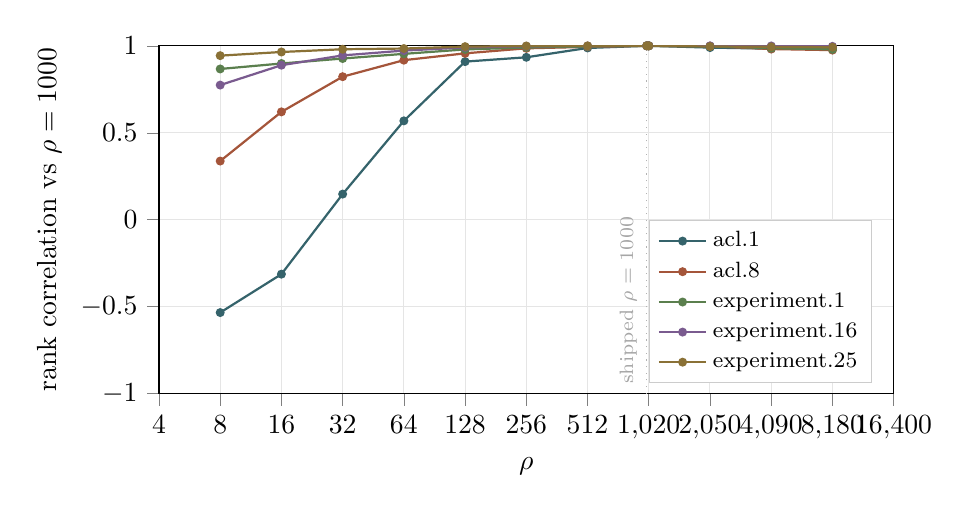
\begin{tikzpicture}
  \definecolor{rhoC0}{HTML}{35636b}
  \definecolor{rhoC1}{HTML}{a4553a}
  \definecolor{rhoC2}{HTML}{5b7f4e}
  \definecolor{rhoC3}{HTML}{7a5b8f}
  \definecolor{rhoC4}{HTML}{8a7136}
  \begin{axis}[
    width=0.9\linewidth, height=6cm,
    xmode=log, log basis x=2, log ticks with fixed point,
    xlabel={$\rho$}, ylabel={rank correlation vs $\rho=1000$},
    ymin=-1, ymax=1,
    grid=major, grid style={gray!20},
    tick align=outside, tick pos=left,
    legend pos=south east, legend cell align=left, legend style={font=\footnotesize, draw=gray!40},
  ]
    \draw[gray!60, dotted] (axis cs:1000,\pgfkeysvalueof{/pgfplots/ymin}) -- (axis cs:1000,\pgfkeysvalueof{/pgfplots/ymax});
    \node[gray!70, font=\scriptsize, anchor=south west, rotate=90] at (axis cs:1000,\pgfkeysvalueof{/pgfplots/ymin}) {shipped $\rho=1000$};
    \addplot[color=rhoC0, mark=*, mark size=1.2pt, thick] coordinates {(8,-0.5335) (16,-0.3127) (32,0.1476) (64,0.5686) (128,0.9092) (256,0.9340) (512,0.9876) (1000,1.0000) (1024,1.0000) (2048,0.9897) (4096,0.9835) (8192,0.9835)};
    \addlegendentry{acl.1}
    \addplot[color=rhoC1, mark=*, mark size=1.2pt, thick] coordinates {(8,0.3375) (16,0.6202) (32,0.8225) (64,0.9174) (128,0.9567) (256,0.9856) (512,0.9938) (1000,1.0000) (1024,1.0000) (2048,0.9979) (4096,0.9814) (8192,0.9752)};
    \addlegendentry{acl.8}
    \addplot[color=rhoC2, mark=*, mark size=1.2pt, thick] coordinates {(8,0.8669) (16,0.8983) (32,0.9269) (64,0.9537) (128,0.9792) (256,0.9902) (512,0.9956) (1000,1.0000) (1024,1.0000) (2048,0.9972) (4096,0.9864) (8192,0.9797)};
    \addlegendentry{experiment.1}
    \addplot[color=rhoC3, mark=*, mark size=1.2pt, thick] coordinates {(8,0.7743) (16,0.8885) (32,0.9449) (64,0.9725) (128,0.9905) (256,0.9974) (512,0.9990) (1000,1.0000) (1024,1.0000) (2048,0.9997) (4096,0.9992) (8192,0.9969)};
    \addlegendentry{experiment.16}
    \addplot[color=rhoC4, mark=*, mark size=1.2pt, thick] coordinates {(8,0.9434) (16,0.9645) (32,0.9802) (64,0.9843) (128,0.9954) (256,0.9990) (512,0.9997) (1000,1.0000) (1024,0.9997) (2048,0.9961) (4096,0.9938) (8192,0.9920)};
    \addlegendentry{experiment.25}
  \end{axis}
\end{tikzpicture}
\caption{Rank correlation of per-cell capability change against the shipped $\rho$, by experiment.}
\label{fig:capability-ratio-per-cell}
\end{figure}

acl.1  (Test Jagged Frontier as published on settings for $\lambda$ AI level fraction $\gamma$ AI dampening (below) as per Stromberg's findings) and acl.8 (Jagged Frontier findings seen as weak) highlight that AI's relative impact on expert performance is stronger than in experiments 1, 16 and 25, which evaluated the impact of AI on expertise, but held the AI leverage function $\ell(E)$ fixed - which creates the strong interactions in the ACL experiments.

For all the experiments the relative outcomes of all parameter settings in the experiments became consistent at $\rho=128$ (a ceiling-to-threshold capability ratio of $128{:}1$), as the convex weighting function $w(E)$ dominates the interaction with $\ell(E)$.

\subsubsection{Graph} \label{sec:Graph}

Two graphs were developed to represent the overall system of institutions.
\begin{itemize}
  \item A BA-Graph (Albert and Barabasi 2002) is generated synthetically and agents are allocated to nodes according to the scale of the node attached to the graph incrementally. The advantage of the BA graph is that the scale of the graph ($M$, the number of nodes), and the density of attachment between the nodes in the graph ($m$, degree of attachment) can be easily controlled and varied in construction allowing for experiments that systematically probe the connectivity and structure of the system as potential factors in AI expertise and capability destruction or amplification. 
  \item A Data Driven Graph that partially models the institutions and structure of the global financial system in 2026.  The data in this graph is a result of individual investigations, estimates and internet scrapes with AI; it should in no way be treated as canonical, but instead is an attempt to describe the modern financial system at a high level to create some information on the applicability of the findings of our work to the real world. The graph used to generate the results in this paper contained data on 330 financial institutions. The data for each institution includes its relative size, estimated graduate/trainee intake, sector (insurance, banking) and presence in the different hub cities.
\end{itemize}
Section \ref{sec:graph_experiments} describes some results from a series of experiments that varied the properties of the BA-Graph creating some interesting results.

\section{Results}\label{sec:results}

A suite of bulk experiments was developed and run to obtain information on the behaviour and interaction of the parameters in the simulation.

\subsection{Evolution of Expertise \& Capability}

Tables \ref{tab:acl-2-meanE-change-t1440} and \ref{tab:acl-2-capabilityChangeFrac-t1440} shows the results from an experiment over combinations of AI learning dampening parameters drawn from \cite{david_stromberg_generative_2026} (see p52, figure A14d.) and expertise moderation/amplification parameters drawn from \cite{fabrizio_dellacqua_navigating_nodate} (see that paper's abstract) across a range of hypothetical AI performance levels. Because Stromberg-et-al.'s experiment addressed high school students the hypothesis for these experiments was that human learning for those above AI competence would suffer no penalties ($\gamma_{\mathrm{above}}$ =0.0).

\begin{table}[htbp]
  \centering
  \caption{Mean expertise, change from no-AI at $t=1440$ months, $\gamma_{\mathrm{below}}$ AI dampening (below) (rows) against $\lambda$ AI level fraction (columns). Grid mean -0.021, range -0.033 to -0.0062. Single-cell noise $\pm 0.0018$ ($2\sigma$, 10 replicates); signal-to-noise 8.8.}
  \label{tab:acl-2-meanE-change-t1440}
  \resizebox{\textwidth}{!}{%
  \begin{tabular}{lrrrrrr}
    \toprule
    $\gamma_{\mathrm{below}}$ AI dampening (below) $\backslash$ $\lambda$ AI level fraction & 0.200 & 0.400 & 0.600 & 0.800 & 0.850 & 0.875 \\
    \midrule
    0.839 & -0.0062 & -0.014 & -0.017 & -0.021 & -0.02 & -0.021 \\
    0.811 & -0.0064 & -0.018 & -0.019 & -0.025 & -0.023 & -0.024 \\
    0.764 & -0.012 & -0.022 & -0.027 & -0.033 & -0.031 & -0.033 \\
    \bottomrule
  \end{tabular}%
  }
\end{table}
Table \ref{tab:acl-2-meanE-change-t1440} shows that at these settings relatively small impacts on the overall expertise in the system can be observed. Human expertise is impaired in the system as would be expected, but the overall dynamics of continual learning and diffusion compensate. However Table \ref{tab:acl-2-capabilityChangeFrac-t1440} shows a more significant impact. The $\ell$ parameter from the Jagged Frontier work, where the performance of junior workers (below AI level) is impaired by their inability to verify results effectively coupled with $\rho$ which expresses the value of high level work amplifies the loss of expertise, and the higher the performance of AI the worse the picture gets, with a potential loss of 16.9\% of capability in the system. It's important to note, two things. First these losses are not monotonic and secondly that's a loss of capability overall \textit{including the boost that having near human level AI to use} would give. 
% acl.2: generated by build_report.js, 2026-08-26T08:35:28.942Z
% requires: \usepackage{booktabs,graphicx}
\begin{table}[htbp]
  \centering
  \caption{Capability, share gained or lost at $t=1440$ months, $\gamma_{\mathrm{below}}$ AI dampening (below) (rows) against $\lambda$ AI level fraction (columns). AI dampening for above expertise = 0.0}
  \label{tab:acl-2-capabilityChangeFrac-t1440}
  \resizebox{\textwidth}{!}{%
  \begin{tabular}{lrrrrrr}
    \toprule
    $\gamma_{\mathrm{below}}$ AI dampening (below) $\backslash$ $\lambda$ AI level fraction & 0.200 & 0.400 & 0.600 & 0.800 & 0.850 & 0.875 \\
    \midrule
    0.839 & 0.0067 & -0.021 & -0.016 & -0.029 & -0.014 & 0.0059 \\
    0.811 & -0.0044 & -0.042 & -0.013 & -0.063 & -0.039 & -0.035 \\
    0.764 & -0.0091 & -0.065 & -0.091 & -0.169 & -0.119 & -0.144 \\
    \bottomrule
  \end{tabular}%
  }
\end{table}

Table\ref{tab:acl-4-capabilityChangeFrac-t1440} shows the results from simulations where AI is assumed to have an impact on humans who have attained expertise above AI ($\gamma_{\mathrm{above}}=0.8$). This scenario is \textbf{unsupported by the empirical results}, but it's not unimaginable that highly expert humans may be as susceptible to the illusion of AI enhanced learning as anyone else. 
% acl.4: generated by build_report.js, 2026-08-26T08:35:28.942Z
% requires: \usepackage{booktabs,graphicx}
\begin{table}[htbp]
  \centering
  \caption{Capability, share gained or lost at $t=1440$ months, $\gamma_{\mathrm{below}}$ AI dampening (below) (rows) against $\lambda$ AI level fraction (columns).}
  \label{tab:acl-4-capabilityChangeFrac-t1440}
  \resizebox{\textwidth}{!}{%
  \begin{tabular}{lrrrrrr}
    \toprule
    $\gamma_{\mathrm{below}}$ AI dampening (below) $\backslash$ $\lambda$ AI level fraction & 0.200 & 0.400 & 0.600 & 0.800 & 0.850 & 0.875 \\
    \midrule
    0.839 & -0.275 & -0.235 & -0.196 & -0.117 & -0.06 & 0.0098 \\
    0.811 & -0.264 & -0.249 & -0.2 & -0.162 & -0.103 & -0.069 \\
    0.764 & -0.303 & -0.262 & -0.265 & -0.227 & -0.161 & -0.177 \\
    \bottomrule
  \end{tabular}%
  }
\end{table}

These results are for epoch t=1440 in the simulation, 120 simulated years of the financial system running on AI. Of course, that's beyond the horizon of concern of most of us, so it's reasonable to check what relevance these results will have on a shorter time scale. 
\begin{figure}[htbp]
  \centering
  \begin{subfigure}[t]{0.48\textwidth}
    \centering
    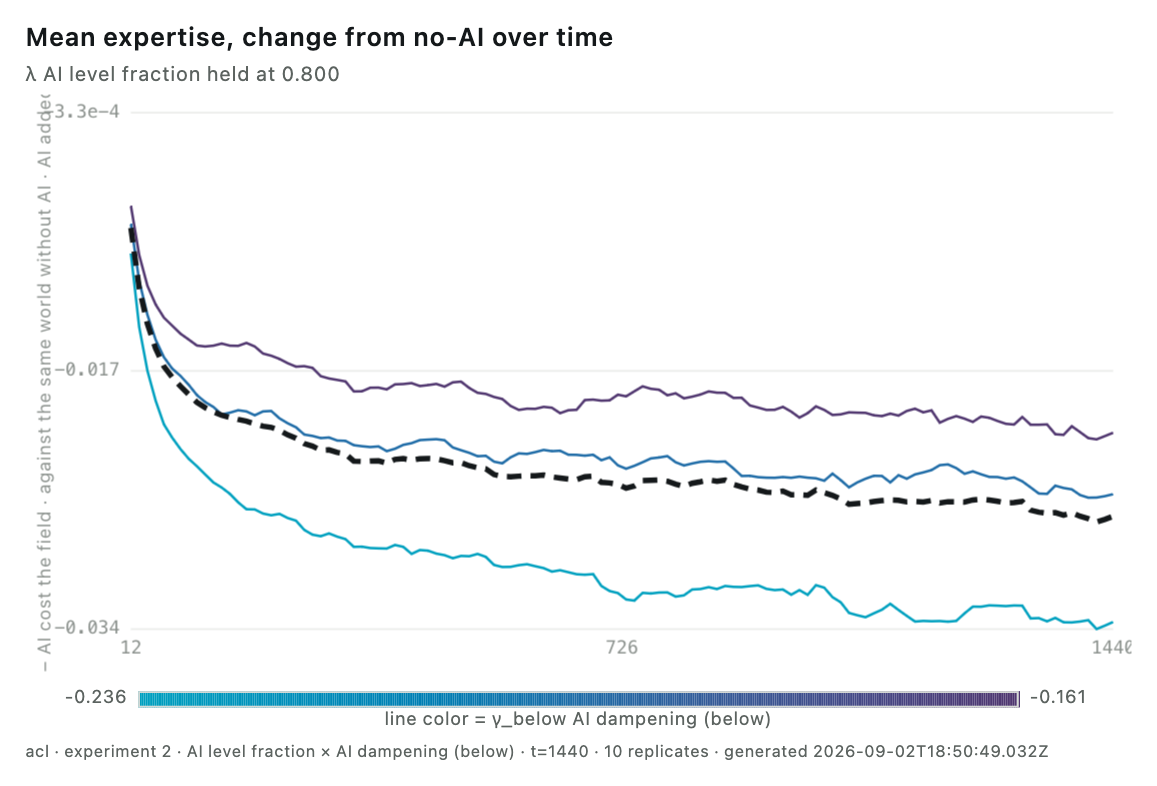
\includegraphics[width=\linewidth]{images/acl-exp2-meanE_change-t1440-panel.png}
    \caption{Mean expertise over time. By 360 ticks (30 years), most of the decline is complete.}
    \label{fig:expertise_decline}
  \end{subfigure}\hfill
  \begin{subfigure}[t]{0.48\textwidth}
    \centering
    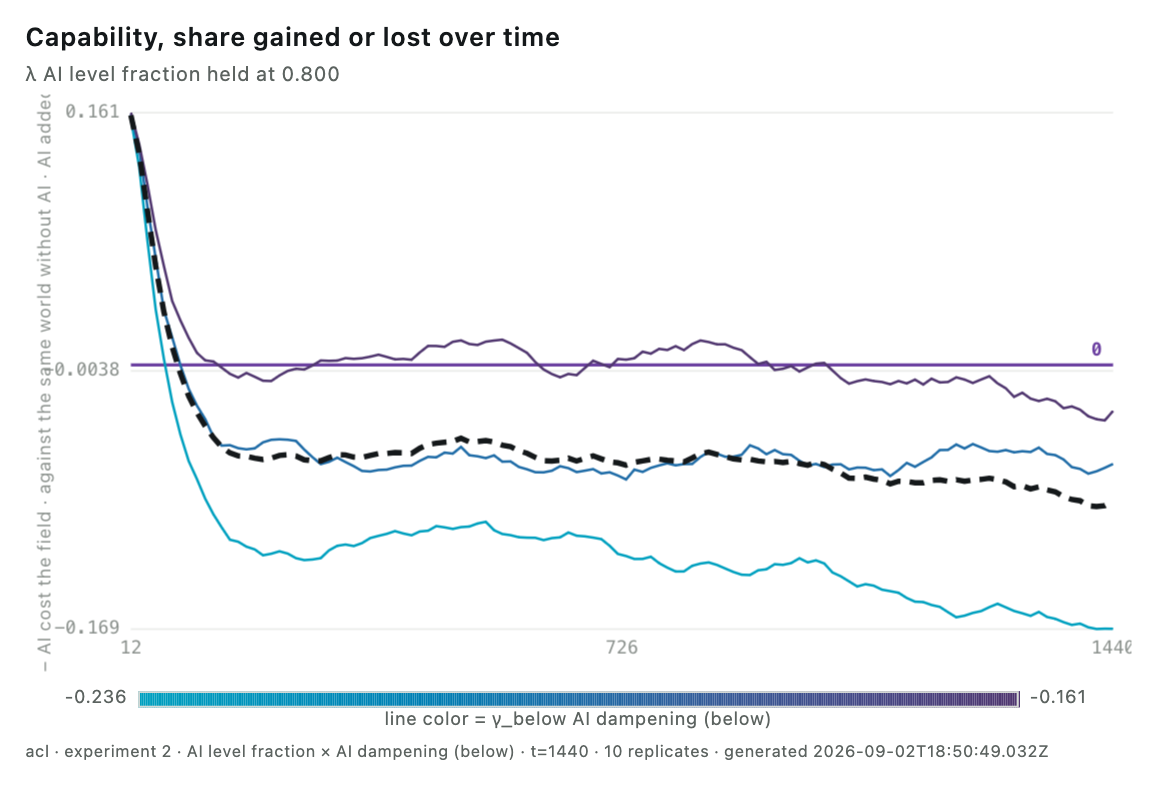
\includegraphics[width=\linewidth]{images/acl-exp2-capabilityChangeFrac-t1440-panel.png}
    \caption{Capability decline is faster as the leverage from $\ell$ and $\rho$ combine}
    \label{fig:capability_decline}
  \end{subfigure}
  \caption{Evolution of expertise and capability during the simulation.} 
  \label{fig:impairment}
\end{figure}
Figures \ref{fig:expertise_decline} and \ref{fig:capability_decline} show the rapid onset of capability decline and stabilisation in these scenarios. 
\subsubsection{Graph Structure Experiments} \label{sec:graph_experiments}
The simulation can be run using two types of description of the structure of the financial system (see section \ref{sec:Graph}), a synthetic graph created using incremental additions of nodes with limited attachment and an AI built graph based on desk research about the constituent elements of the system and a model of employment mobility. The purpose of the synthetic graph is to enable exploration of the impact of these structures. A number of experiments were run varying the properties $M$ (node count) and $m$ (attachment count) and measuring whether these made any difference to the evolution of expertise and capability. Nine experiments checking the interaction of settings for AI parameters and the graph structure parameters were run: $\lambda \times M$, $\lambda \times m$, $\gamma_{\mathrm{below}} \times M$, $\gamma_{\mathrm{below}} \times m$, $\gamma_{\mathrm{above}} \times M$, $\gamma_{\mathrm{above}} \times m$, $\beta \times M$, $\beta \times m$, and $M \times m$.

In Table \ref{tab:structure-3-capabilityChangeFrac-t1440} we see that $\gamma_{\mathrm{below}}$ dominates as a performance driver, but graph structure is significant. Values of $M$ drive variations in outcome of as much as 18.5\% where dampening is high ($\gamma_{\mathrm{below}} =0.2$). 
% structure.3: generated by build_report.js, 2026-09-07T20:53:24.117Z
% requires: \usepackage{booktabs,graphicx}
\begin{table}[htbp]
  \centering
  \caption{Capability, share gained or lost at $t=1440$ months, $M$  m (rows) against $\gamma_{\mathrm{below}}$ AI dampening (below) (columns). Grid mean -0.073, range -1 to 0.37. Single-cell noise $\pm 0.008$ ($2\sigma$, 32 replicates)}
  \label{tab:structure-3-capabilityChangeFrac-t1440}
  \resizebox{\textwidth}{!}{%
  \begin{tabular}{lrrrrrrrrrrrrrrrrrrrrr}
    \toprule
    $M$  m $\backslash$ $\gamma_{\mathrm{below}}$ AI dampening (below) & 0.0 & 0.1 & 0.2 & 0.3 & 0.4 & 0.5 & 0.6 & 0.7 & 0.8 & 0.9 & 1.0 & 1.1 & 1.2 & 1.3 & 1.4 & 1.5 & 1.6 & 1.7 & 1.8 & 1.9 & 2.0 \\
    \midrule
    132 & -1 & -0.999 & -0.906 & -0.652 & -0.446 & -0.292 & -0.179 & -0.092 & -0.0027 & 0.047 & 0.1 & 0.151 & 0.19 & 0.22 & 0.248 & 0.264 & 0.302 & 0.312 & 0.328 & 0.359 & 0.37 \\
    109 & -1 & -0.998 & -0.889 & -0.639 & -0.431 & -0.28 & -0.178 & -0.083 & -0.004 & 0.056 & 0.1 & 0.149 & 0.175 & 0.219 & 0.227 & 0.267 & 0.285 & 0.301 & 0.313 & 0.345 & 0.342 \\
    90 & -1 & -0.997 & -0.876 & -0.605 & -0.408 & -0.254 & -0.145 & -0.074 & -0.0039 & 0.061 & 0.1 & 0.147 & 0.171 & 0.212 & 0.236 & 0.266 & 0.276 & 0.295 & 0.305 & 0.332 & 0.367 \\
    75 & -1 & -0.995 & -0.861 & -0.595 & -0.393 & -0.252 & -0.15 & -0.059 & 0.0017 & 0.055 & 0.1 & 0.138 & 0.176 & 0.195 & 0.236 & 0.257 & 0.273 & 0.289 & 0.302 & 0.317 & 0.341 \\
    62 & -1 & -0.992 & -0.845 & -0.579 & -0.383 & -0.241 & -0.133 & -0.062 & 0.0076 & 0.055 & 0.1 & 0.132 & 0.176 & 0.208 & 0.231 & 0.247 & 0.277 & 0.285 & 0.288 & 0.319 & 0.32 \\
    51 & -1 & -0.989 & -0.832 & -0.565 & -0.364 & -0.224 & -0.145 & -0.066 & 0.0075 & 0.061 & 0.1 & 0.143 & 0.167 & 0.188 & 0.221 & 0.241 & 0.256 & 0.266 & 0.28 & 0.29 & 0.323 \\
    42 & -1 & -0.986 & -0.818 & -0.557 & -0.363 & -0.228 & -0.122 & -0.065 & 0.0074 & 0.056 & 0.1 & 0.132 & 0.172 & 0.201 & 0.209 & 0.234 & 0.245 & 0.271 & 0.286 & 0.292 & 0.301 \\
    35 & -0.999 & -0.984 & -0.813 & -0.54 & -0.353 & -0.21 & -0.136 & -0.055 & 0.019 & 0.051 & 0.1 & 0.137 & 0.158 & 0.184 & 0.209 & 0.224 & 0.254 & 0.268 & 0.266 & 0.304 & 0.312 \\
    29 & -0.999 & -0.98 & -0.8 & -0.523 & -0.338 & -0.213 & -0.113 & -0.045 & 0.022 & 0.059 & 0.1 & 0.134 & 0.173 & 0.2 & 0.212 & 0.226 & 0.246 & 0.276 & 0.273 & 0.285 & 0.295 \\
    24 & -0.998 & -0.974 & -0.786 & -0.52 & -0.332 & -0.204 & -0.111 & -0.043 & 0.015 & 0.061 & 0.1 & 0.133 & 0.161 & 0.184 & 0.208 & 0.227 & 0.243 & 0.257 & 0.271 & 0.282 & 0.292 \\
    20 & -0.997 & -0.971 & -0.781 & -0.511 & -0.324 & -0.2 & -0.11 & -0.041 & 0.016 & 0.062 & 0.1 & 0.133 & 0.16 & 0.183 & 0.204 & 0.223 & 0.238 & 0.254 & 0.267 & 0.281 & 0.29 \\
    16 & -0.996 & -0.964 & -0.769 & -0.501 & -0.318 & -0.197 & -0.108 & -0.037 & 0.016 & 0.062 & 0.1 & 0.132 & 0.159 & 0.181 & 0.202 & 0.221 & 0.236 & 0.251 & 0.264 & 0.278 & 0.288 \\
    14 & -0.995 & -0.962 & -0.761 & -0.496 & -0.313 & -0.191 & -0.105 & -0.035 & 0.019 & 0.064 & 0.1 & 0.132 & 0.158 & 0.181 & 0.201 & 0.22 & 0.234 & 0.25 & 0.262 & 0.273 & 0.284 \\
    11 & -0.993 & -0.957 & -0.75 & -0.489 & -0.308 & -0.189 & -0.103 & -0.033 & 0.019 & 0.064 & 0.1 & 0.131 & 0.157 & 0.18 & 0.201 & 0.218 & 0.232 & 0.247 & 0.26 & 0.267 & 0.281 \\
    9 & -0.992 & -0.952 & -0.748 & -0.484 & -0.309 & -0.187 & -0.098 & -0.033 & 0.02 & 0.063 & 0.1 & 0.13 & 0.157 & 0.179 & 0.201 & 0.217 & 0.232 & 0.246 & 0.26 & 0.269 & 0.278 \\
    8 & -0.99 & -0.951 & -0.746 & -0.479 & -0.302 & -0.186 & -0.097 & -0.033 & 0.021 & 0.064 & 0.1 & 0.13 & 0.156 & 0.179 & 0.198 & 0.215 & 0.232 & 0.243 & 0.256 & 0.268 & 0.279 \\
    6 & -0.987 & -0.944 & -0.74 & -0.472 & -0.3 & -0.181 & -0.097 & -0.033 & 0.022 & 0.064 & 0.1 & 0.13 & 0.156 & 0.178 & 0.197 & 0.215 & 0.229 & 0.245 & 0.256 & 0.266 & 0.277 \\
    5 & -0.985 & -0.942 & -0.733 & -0.47 & -0.296 & -0.178 & -0.093 & -0.031 & 0.022 & 0.064 & 0.1 & 0.13 & 0.155 & 0.179 & 0.196 & 0.214 & 0.229 & 0.243 & 0.255 & 0.267 & 0.276 \\
    4 & -0.983 & -0.937 & -0.734 & -0.467 & -0.295 & -0.178 & -0.094 & -0.028 & 0.023 & 0.065 & 0.1 & 0.13 & 0.154 & 0.177 & 0.197 & 0.214 & 0.227 & 0.241 & 0.252 & 0.265 & 0.274 \\
    3 & -0.98 & -0.935 & -0.726 & -0.468 & -0.294 & -0.176 & -0.093 & -0.027 & 0.022 & 0.065 & 0.1 & 0.129 & 0.154 & 0.177 & 0.197 & 0.214 & 0.23 & 0.24 & 0.253 & 0.264 & 0.276 \\
    \bottomrule
  \end{tabular}%
  }
\end{table}

Figure \ref{fig:M_as_a_variable} shows two trajectories for values of interest ($\gamma_{\mathrm{below}}$ -0.2/0.8 vs -0.4/0.6) in \ref{tab:structure-3-capabilityChangeFrac-t1440}, note that the y-axis for each graph is different because the range of values generated in the simulation is wider at -0.4/0.6 than at -0.2/0.8. There is a monotonic relationship between the outcomes of the simulation and the structure of the graph (in terms of $M$), graphs with more nodes, and therefore a greater dispersal of expertise fail to generate experts over time. This failure leads to a drop of teaching capability and dispersed system structures settle to lower expertise and lower capability leverage. 

\begin{figure}[htbp]
  \centering
  \begin{subfigure}[t]{0.48\textwidth}
    \centering
    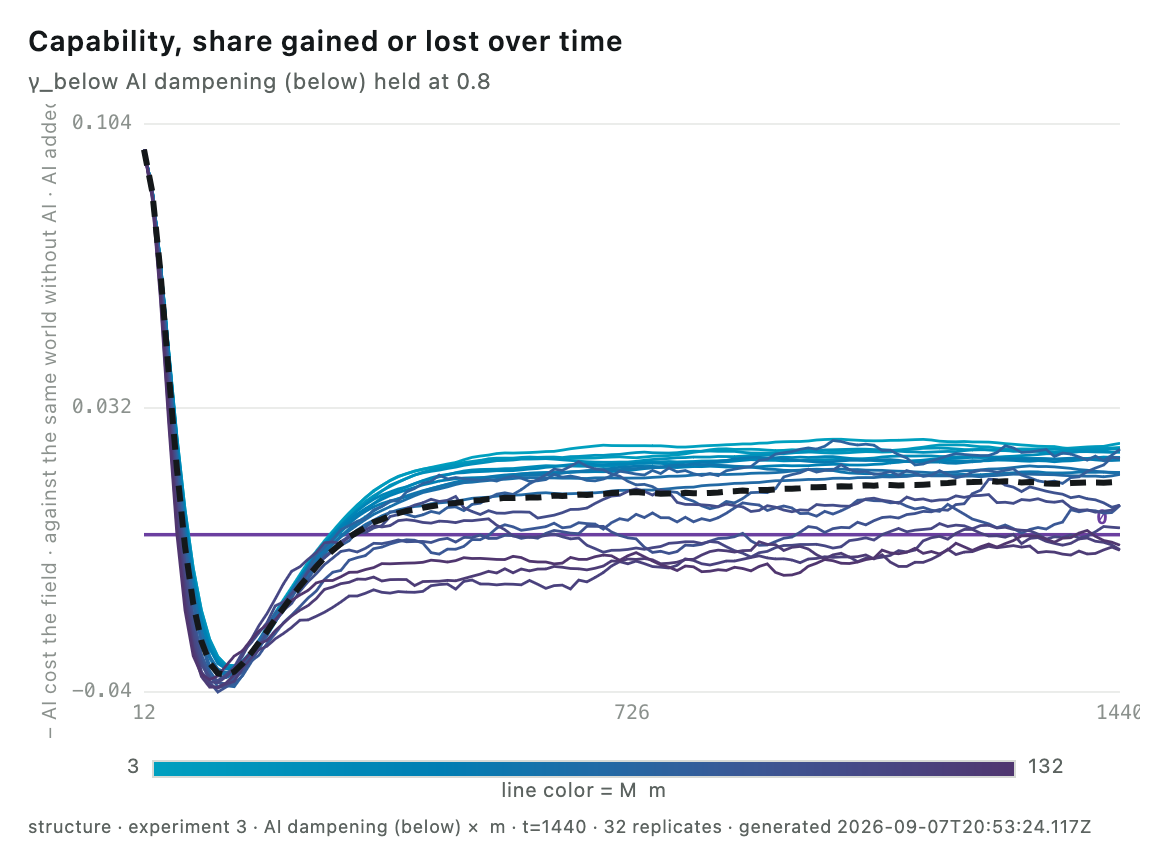
\includegraphics[width=\linewidth]{images/structure-exp3-capabilityChangeFrac-t1440-panelA.png}
    \label{fig:m_breakout.png}
  \end{subfigure}\hfill
  \begin{subfigure}[t]{0.48\textwidth}
    \centering
    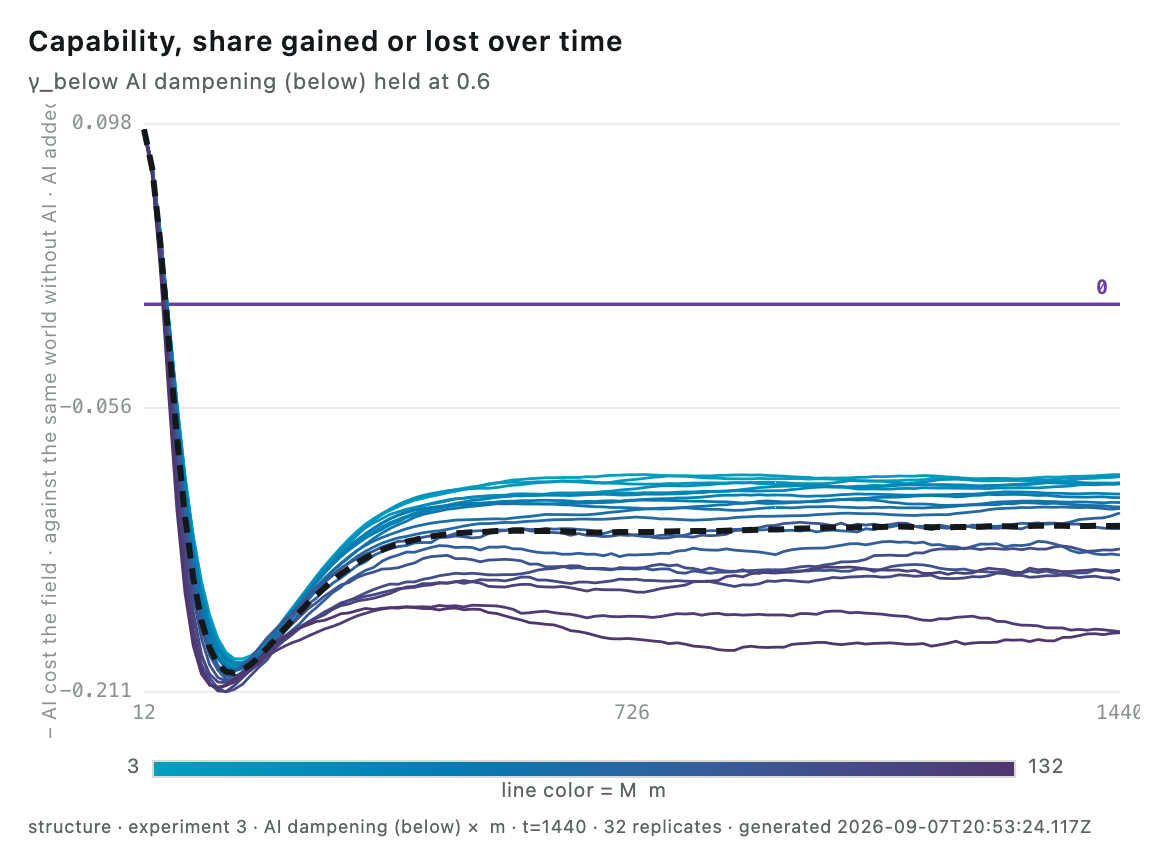
\includegraphics[width=\linewidth]{images/structure-exp3-capabilityChangeFrac-t1440-panelB.png}
    \label{fig:m_smooth}
  \end{subfigure}
  \caption{Comparing the behaviour of simulations with values of $M$ at different levels of AI dampening for agents below AI capability levels $\gamma_{\mathrm{below}}$ -0.2/0.8 vs -0.4/0.6}
  \label{fig:M_as_a_variable}
\end{figure}


\FloatBarrier
\subsubsection{Events Experiments}

The Global Financial System is prone to shocks and sudden shifts. For example the crash of 1929, the end of the gold standard under Nixon and the Global Financial Crisis of 2008. Is AI creating a new shock? Recent press reports have created speculation that AI is a causative factor in a possible reduction of new entrant recruitment \footnote{https://www.thebanker.com/content/8b2ab738-b37c-4bf5-8ce1-75423d147ab8} \footnote{https://www.dallasfed.org/research/economics/2026/0901}. To investigate the potential impact of this reaction to the introduction of AI into the Financial System a set of experiments were created to test the impact of a five year hiring freeze, or reduction on the simulated system. Freeze intensities were varied between 90\% of retirees being replaced and 10\% of retirees being replaced. The impact of the freeze vs. AI learning dampening ($\gamma_{\mathrm{below}}$, $\gamma_{\mathrm{above}}$, and AI performance ($\lambda$) was tested). 

\begin{figure}[htbp]
  \centering
  \begin{subfigure}[t]{0.48\textwidth}
    \centering
    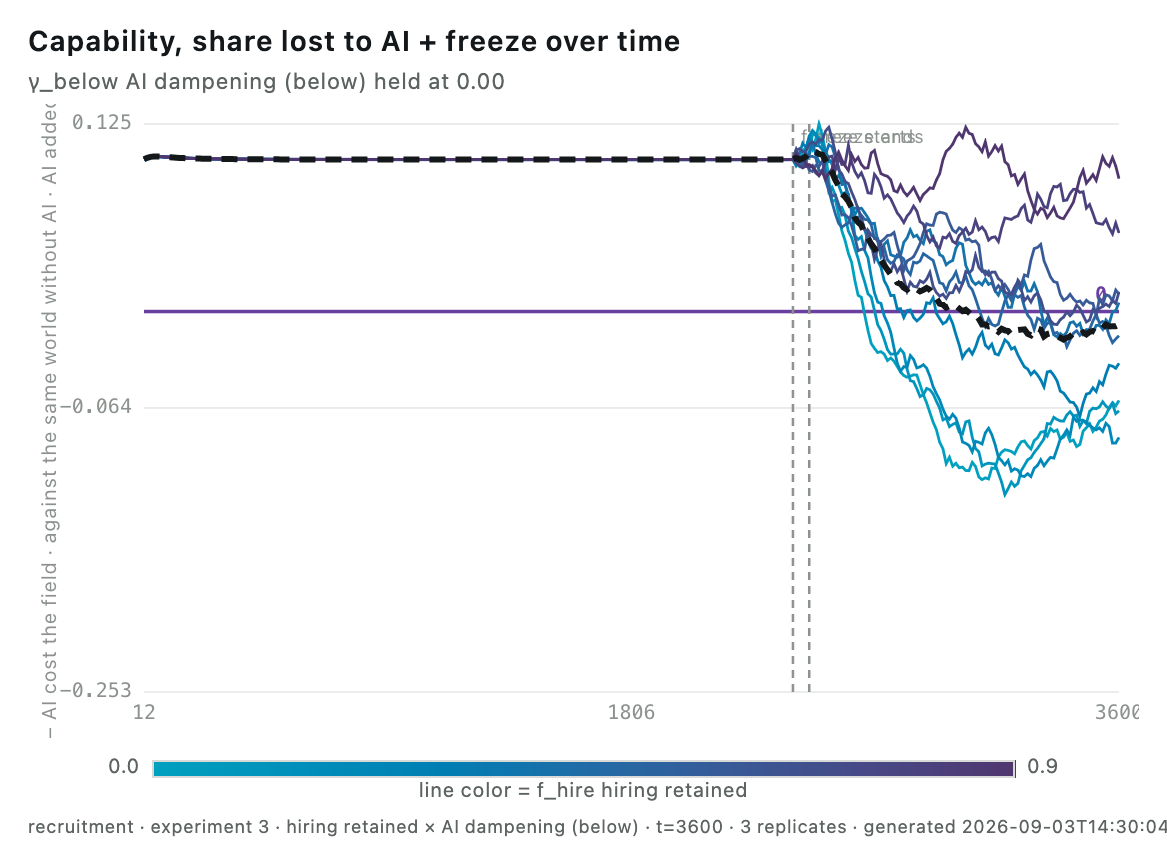
\includegraphics[width=\linewidth]{images/recruitment-exp3-capabilityChangeFrac-t3600-0-0.png}
    \caption{Impact of the hiring freeze when $\gamma_{\mathrm{below}}$ 0.0 - no suppression, and $\lambda$ is set to 0.585}
    \label{fig:shock_00}
  \end{subfigure}\hfill
  \begin{subfigure}[t]{0.48\textwidth}
    \centering
    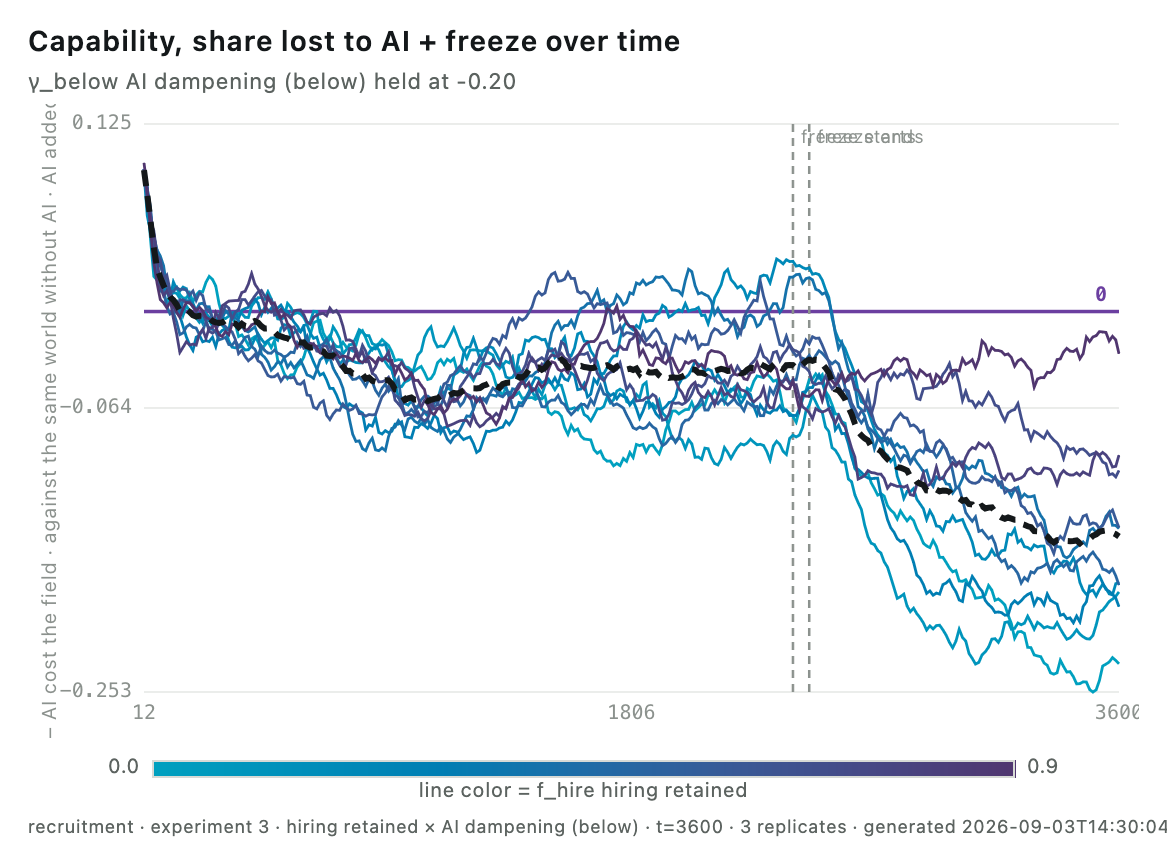
\includegraphics[width=\linewidth]{images/recruitment-exp3-capabilityChangeFrac-t3600-0-2.png}
    \caption{Impact of the hiring freeze when ($\gamma_{\mathrm{below}}$ is set to 0.2 and $\lambda$ is set at 0.585}
    \label{fig:shock_02}
  \end{subfigure}
  \caption{The impact of hiring freezes on an AI enabled system where (a) there is no learning suppression, and (b) there is minimal learning suppression.}
  \label{fig:two_shock}
\end{figure}

Figure \ref{fig:two_shock} shows the impact of freezes on the system with and without learning dampening. Because the same number of random processes is being run in the AI vs no AI arms of the simulator when $\gamma_{\mathrm{below}}$ is 0.0 and no freeze has occurred there is no divergence for the population in \ref{fig:shock_00} until the freeze epoch is hit. Then the different levels of retention in play result in significant divergence which persists for many epochs. The results are less stark for \ref{fig:shock_02} with the populations generating more diversity due to learning suppression being active before the freeze hits. When the freeze occurs a similar set of declines is observed but in this case it is noticeable, but not unexpected, that some of the populations with higher retention values appear more resilient to the shock. 

\subsection{Limitations}

The most important limitation of this work is that it is ``only'' a simulation and the dynamics are the dynamics chosen and implemented by its creators. It is obviously not possible to claim that this work faithfully, or comprehensively recreates the dynamics of learning and performance in the real world of financial services or any other human knowledge institution. The study should be read as an investigation into a possible world rather than a prediction about the real world. 

Two versions of the simulator were implemented, one using a degree 2 BA-graph \cite{albert_statistical_2002} and one using a graph that is derived with a set of assumptions from real world information about the distribution and scale of financial institutions in 2026. This model should be taken as a ``best guess'' of what the global financial system looks like at the top level, rather than a canonical description. 

The model is scaled 1:200 with one agent representing $200$ employees in the institutions. This potentially introduces more fragility and might suppress or rule out microscale dynamics that could then propagate to affect the simulation on a macro scale. 

 Another criticism of the simulation and model that underpins it is that it is complicated and over-parameterised. A number of parameters were introduced into the model in a successful attempt to produce stable behaviour in the non-AI case. For example the $S$ parameter for post teaching threshold was required to prevent collapses in $E_n$ due to top end attrition of expert agents over time. However, multiple parameter simulations can potentially be tuned to demonstrate the results that their users are fishing for.

 Our assumptions also should be examined. The simulator considers learning penalties as compounding, so while \cite{david_stromberg_generative_2026} and others have measured singular events demonstrating a fall off of learning performance the simulator assumes that this is a recurrent penalty. The same is true for the Jagged Frontier assumptions \cite{fabrizio_dellacqua_navigating_nodate}, the leverage there is seen and used in the simulator as a fixed penalty or boost, the possibility of human adaptation is not anticipated in this work. 

\section{Recommendations} \label{sec:recommendations}

Despite the criticism that can be made of the model and simulator and the limitations of the investigations of its behaviour to date there are some observations to be made about the observed results.

\begin{itemize}
  \item When the simulation is parameterised with the values observed by \cite{david_stromberg_generative_2026} and \cite{fabrizio_dellacqua_navigating_nodate} rapid and significant losses to systemic capability are seen \ref{fig:impairment} 
  \item A new entrant hiring reduction (of the type that may be underway currently) has large and long term impacts even in the case where AI is not simulated as suppressing learning. It should be emphasised that this impact is despite the fact that the calculation of overall capability accounts for the uplift from AI. 
\end{itemize}
There are possible mitigations that could avoid some of these issues. The recent study \cite{fan_beware_2025} identified a potential mechanism that may drive reduction of learning by AI users (despite not finding that reduction in their study). The reduction of meta-cognitive behaviours during learning might be interpreted as the loss of skill that impairs the development of expertise. Financial services institutions might be able to repair some of this lack by either selecting candidates for metacognitive behaviours or by providing specific training on these practices. Selection for these behaviours could be done using roleplaying or team exercises in assessment centres. 

With respect to the impact of the hiring freeze the obvious remedy was prescribed by Matt Garman of Amazon who said that: \begin{quotation}
replacing entry-level staff with AI tools is ``one of the dumbest things I've ever heard.''
\end{quotation} and went on to say companies should keep hiring graduates and teaching them how to build software, break down problems, and adopt best practices \footnote{https://www.businessinsider.com/amazon-cloud-chief-replacing-junior-staff-ai-matt-garman-2025-8}. Unfortunately Garman is speaking and acting from a position of comfort. Financial services leaders operating in a fiercely competitive environment with shareholders insisting on a return on capital will be driven to take what options they can identify to cut costs and drive returns. A recent study \cite{falk_ai_2026} discusses staff reductions as a dominant strategy for organisations responding to the availability of modern AI. While agreeing with the analysis presented in ``The Layoff Trap'' we do not agree with the prescription of a taxation based approach to change motivations. Instead society has a strong response which it can use to create a countervailing force. This is regulation; regulators can insist that FSIs report on and maintain human capital plans, these should require that talent pipelines and comprehensive training for staff are provided. 

It's important that this is not an untried approach, for hundreds of years a stable system of guild regulation and skill management persisted in economies all over the world. We believe this is a good fit as a social response in the face of a world of work where there will be less opportunity to learn by doing. Practically speaking, rather than simply creating guilds,  FSIs could be required to build simulations and assessments that force junior workers to demonstrate their "no AI" capabilities, especially highlighting meta-cognition. We're used to the idea that militaries train and drill so that they are ready for war, the idea that banks will drill and train so as to be ready for a crisis where AI doesn't have all the answers is not so alien. 

A simple pushback to this line of argument is to ask "what does it matter if the expertise and capability in the system drops? After all, we will have better and better AI, perhaps AGI." AI as it exists now is a backwards looking technology, the models are fashioned from history. Humans learn skills and ways of thinking that are applicable in novel situations, and while it could be the case that AGI is able to cope with a great many novel situations it may be the case that something comes up that it can't cope with, and in that case we might all heartily wish that we had maintained the ability to deal with whatever surprises pop out of the woodwork ourselves. 

\section{Conclusion}

Psychological and cultural impacts created by GenAI and Agent systems as a mode of risk to a system are insidious, because these risks may be hard to detect, and tempting to elide. These risks threaten long term and persistent harms as individuals and institutions may come to lack the capabilities to redevelop or reconstruct skills, norms, and capabilities, that they have lost. Indeed, it may be that over time even the ability to conceive of the loss is, itself, lost. Potentially we may be left with a financial system that fails, is unable to reconstruct itself, and cannot understand what has happened to it.
It hardly needs to be said; this would not be an optimal outcome.

\bibliographystyle{plainnat}
\bibliography{my_library}


\section*{Parameter Glossary}

\begingroup
\setlength{\tabcolsep}{3pt}
\noindent\footnotesize
\begin{longtable}{L{1.6cm} K{3.8cm} L{6.9cm} S{3.2cm}}
\toprule
\textbf{Symbol} & \textnormal{\textbf{Parameter}} & \textbf{Definition} &
\textbf{Default} \\
\midrule
\endfirsthead
\toprule
\textbf{Symbol} & \textnormal{\textbf{Parameter}} & \textbf{Definition} &
\textbf{Default} \\
\midrule
\endhead
\bottomrule
\endlastfoot
\multicolumn{4}{@{}l}{\itshape Scale}\\[2pt]
$N$ & N & Population size, number of agents in simulation.
  & $500$\newline {\scriptsize $11322$ world model} \\
$M$ & M & Number of institutions .
  & $40$ \\
$T$ & horizon & Ticks (months) to simulate; $1440$ is three careers.
  & $1440$ \\
\addlinespace
\multicolumn{4}{@{}l}{\itshape Initial expertise --- $t=0$ population only}\\[2pt]
$\mu_E$ & expertiseMean & Location of the starting skew-normal skill draw.
  & $0.28$ \\
$\omega_E$ & expertiseSpread & Scale of that draw, before clipping to $[0,1]$.
  & $0.30$ \\
$\alpha_E$ & expertiseSkew & Shape; positive thins the low tail.
  & $3$ \\
\addlinespace
\multicolumn{4}{@{}l}{\itshape Entrants --- turnover replacements}\\[2pt]
$\mu_{\text{ent}}$ & entrantExpertiseMean & Mean skill of a recruit replacing a
  retiree --- deliberately low, so entrants are genuine novices.
  & $0.05$ \\
$\omega_{\text{ent}}$ & entrantExpertiseSpread & Spread of recruit skill.
  & $0.05$ \\
$E_{\min}$ & entrantExpertiseFloor & Hard lower bound applied \emph{after}
  clipping the draw, so entrants do not pile up at exactly $0$.
  & $0.05$ \\
\addlinespace
\multicolumn{4}{@{}l}{\itshape Institution graph}\\[2pt]
$m$ & graphAttachment & Barab\'asi--Albert edges per new node --- controls how
  sharply hub institutions form.
  & $2$ \\
\addlinespace
\multicolumn{4}{@{}l}{\itshape Learning \& decay}\\[2pt]
$\beta$ & transferRate & Monthly fraction of the gap to the teaching level closed
  by peer learning.
  & $0.15$\newline {\scriptsize raw $0.5$} \\
$\delta$ & decayRate & Monthly rate expertise erodes when at or above the
  teaching level.
  & $0.020$\newline {\scriptsize pipeline $0.027$} \\
$\sigma_L$ & learningRateSpread & Spread of the lognormal per-person multiplier
  $L_i$; $0 = $ everyone identical.
  & $0.4$\newline {\scriptsize $1.0$ world model} \\
$c$ & learningCap & Ceiling on expertise gained per tick from peers, before
  $L_i$; makes the climb linear rather than exponential.
  & $0$ (off)\newline {\scriptsize pipeline $0.0056$} \\
$T_s$ & seniorTenureYears & Years in the field before a member counts toward what
  trainees learn from.
  & $0$ (off)\newline {\scriptsize pipeline $8$} \\
$\mu_p$ & personalLearningRate & Monthly self-improvement once no gap remains;
  scaled by the institution's founding mean. May be negative.
  & $0.001$ \\
$\omega_a$ & aptitudeSpread & Spread of per-person ceilings on attainable
  expertise, drawn at entry; $0 = $ no ceiling.
  & $0$ (off)\newline {\scriptsize pipeline $0.20$} \\
$n_t$ & teachTopN & Number of top seniors whose mean sets the teaching level ---
  an absolute count, not a percentile.
  & $0$ (off)\newline {\scriptsize $8$ pipeline / WM} \\
$k_d$ & aboveMeanDrag & Brake dividing a learning delta by
  $1 + k_d(E_i - \bar E)$ above the population mean; only ever slows learning.
  & $0$ (off)\newline {\scriptsize pipeline $16$} \\
$n_0$ & criticalMass\dg & Expert count an institution needs to transfer at full
  efficiency; $0 = $ off.
  & $0$ (off) \\
$h$ & criticalMassSharpness\dg & Hill exponent for the critical-mass falloff;
  ${\sim}1$ gentle, $\ge 8$ a hard cutoff.
  & $2$ \\
\addlinespace
\multicolumn{4}{@{}l}{\itshape Mobility}\\[2pt]
\dither & mobilityMode & Candidate-set rule: \texttt{unconstrained} /
  \texttt{edge\_constrained} / \texttt{hybrid}.
  & hybrid \\
$\kappa$ & competitionAversion & Weight on relative standing vs.\ room to grow in
  the move utility. 
  & $0.5$ \\
$\eta$ & prestigeWeight & Weight on an institution's structural prestige (its
  degree).
  & $0.3$ \\
$p_{\text{move}}$ & baseMoveProb & Base monthly probability of reconsidering
  institution; scaled per person by $L_i$.
  & $0.05$\newline {\scriptsize $0.01$ world model} \\
$\varepsilon$ & jumpProbability & Hybrid mode: chance the candidate set is drawn
  from the whole graph rather than local neighbours.
  & $0.10$ \\
$\tau$ & MOVE\_TEMPERATURE\dg & Softmax temperature for the destination draw;
  fixed in \texttt{engine.js}.
  & $0.12$ \\
\addlinespace
\multicolumn{4}{@{}l}{\itshape Turnover \& recruitment shock}\\[2pt]
$r$ & turnoverRate & Monthly retire-and-replace probability,
  $= 1/\text{career-months}$. $N$, this and career length are one identity.
  & $1/480 \approx 0.00208$ \\
\dither & recruitmentShockStart & Tick a hiring freeze begins.
  & $0$ \\
\dither & recruitmentShockYears & Length of the freeze, in years; $0 = $ off.
  & $0$ (off) \\
\dither & recruitmentFraction & Share of retirements still refilled during the
  freeze; $1 = $ no freeze.
  & $1$ \\
\addlinespace
\multicolumn{4}{@{}l}{\itshape AI mechanism}\\[2pt]
$\lambda$ & aiLevelFraction & AI strength as a fraction of the $t=0$ top human;
  sets the absolute level $A$. $0.585 = $ ``as good as an expert''.
  & $0.585$ \\
$\gamma_{\text{below}}$ & aiDampeningBelow & Multiplier on learning for people
  \emph{below} $A$: $0 = $ zeroed out, $1 = $ neutral, $2 = $ doubled.
  & $0.30$ \\
$\gamma_{\text{above}}$ & aiDampeningAbove & The same multiplier for people at or
  above $A$; bites only when such people exist.
  & $0.80$ \\
$b$ & frontierBreadth & Exponent setting the in-frontier work share $F = A^{b}$;
  lower widens the AI's reach.
  & $1$ \\
$g_n$ & aclNoviceGain\dg & In-frontier output gain for weaker performers.
  & $0.43$ \\
$g_x$ & aclExpertGain\dg & In-frontier output gain for stronger performers.
  & $0.17$ \\
$d_n$ & aclNoviceDeficit\dg & Out-of-frontier output loss for those who cannot
  catch the AI's errors.
  & $0.19$ \\
$s$ & aclBlendSharpness\dg & How sharply the novice and expert leverage regimes
  blend across $E$; large values approach a hard bin.
  & $20$ \\
\addlinespace
\multicolumn{4}{@{}l}{\itshape Fixed constants --- \texttt{engine.js}}\\[2pt]
$\theta$ & EXPERT\_THRESHOLD & Expertise at or above which someone counts as an
  expert; anchors $w(\theta) = 1$ and \texttt{shareExpert}.
  & $0.585$ \\
$\rho$ & CAPABILITY\_RATIO & How many threshold-experts one person at $E = 1$ is
  worth.
  & $1000$ \\
\end{longtable}

\normalsize
{\footnotesize\noindent\dag\ Not exposed as a slider in \texttt{simulator.html}
--- engine default, or swept only in the batch experiment sets.\par}

% =====================================================================
\section*{Derived \& emergent quantities}

\noindent Computed each tick from the parameters and the current state --- not
set directly.

\medskip
\noindent\footnotesize
\begin{longtable}{L{1.9cm} K{3.4cm} L{7.3cm}}
\toprule
\textbf{Symbol} & \textnormal{\textbf{Source}} & \textbf{Meaning} \\
\midrule
\endfirsthead
\toprule
\textbf{Symbol} & \textnormal{\textbf{Source}} & \textbf{Meaning} \\
\midrule
\endhead
\bottomrule
\endlastfoot
$A$ & aiLevel & Absolute AI level, $\lambda \cdot \max_i E_i(0)$.
  \\
$L_i$ & \textnormal{per person} & Individual multiplier on learning, decay and
  mobility.
  \\
$a_i$ & aptitude & Person $i$'s ceiling on attainable expertise.
  \\
$\bar E_j$ & Ebar & Institution $j$'s current mean expertise.
  \\
$\bar E_j^{\,0}$ & startEbar & Institution $j$'s \emph{founding} mean, fixed at
  $t = 0$ --- anchor for ambient learning.
  \\
$\bar E$ & \textnormal{live} & Population mean expertise at the start of the tick
  --- reference for the above-mean drag.
  \\
$T_j$ & Teach & Institution $j$'s teaching level --- what its trainees climb
  toward.
  \\
$x_j$ & \textnormal{count} & Number of experts ($E \ge \theta$) in institution
  $j$.
  \\
$\varphi_j$ & transferEff & Institution's transfer / production efficiency --- a
  Hill function of $x_j$.
  \\
$P_j$ & prestige & Normalised degree of institution $j$, fixed at graph creation.
  \\
$w(E)$ & capabilityWeight & Per-person expertise $\rightarrow$ value weight, in
  threshold-expert equivalents.
  \\
$\ell(E)$ & aclLeverage & Per-person AI capability multiplier; $1$ when AI is off.
  \\
\end{longtable}
\endgroup

\sloppy

\end{document}
